\documentclass[10pt,a4paper]{article}
\usepackage[a4paper,left=16.5mm,right=16.5mm,top=16mm,bottom=18mm,columnsep=5mm]{geometry}
\usepackage{newtxtext}
\usepackage{newtxmath}
\usepackage{graphicx}
\usepackage{booktabs}
\usepackage{amsmath}
\usepackage{titlesec}
\usepackage{adjustbox}
\usepackage{microtype}
\usepackage{multicol}
\usepackage{xurl}
\graphicspath{{figures/}}
\titleformat{\section}{\normalfont\normalsize\centering}{}{0pt}{}
\titleformat{\subsection}{\normalfont\normalsize\itshape}{}{0pt}{}
\titlespacing*{\section}{0pt}{0.85em}{0.4em}
\titlespacing*{\subsection}{0pt}{0.65em}{0.3em}
\setlength{\parskip}{0pt}
\setlength{\parindent}{1em}
\renewcommand{\baselinestretch}{1.05}
\raggedbottom
\setlength{\emergencystretch}{2em}
\setlength{\columnsep}{5mm}
\setlength{\multicolsep}{7pt}
\begin{document}
\normalsize
\begin{center}
{\fontsize{20}{24}\selectfont When Overall AUC Hides Miscalibration - Evaluating Knowledge Tracing on Rarely Practiced Knowledge Components\par}
\vspace{22pt}
{\fontsize{11}{13}\selectfont Khanh-Trinh Nguyen$^{1}$, Tuan Dao Minh$^{1}$, Duong Nguyen Tien$^{1}$, Chi Thanh Nguyen$^{2}$, and Van-Hau Nguyen$^{1}$,$^{*}$\par}
\vspace{0.25em}
{\fontsize{9}{11}\selectfont $^{1}$ Hung Yen University of Technology and Engineering, Hung Yen, Vietnam\\
$^{2}$ Academy of Military Science and Technology, Ha Noi, Vietnam\\
Email: trinhnk@utehy.edu.vn (K.-T.N.); tuanymc@utehy.edu.vn (T.D.M.); duongnt@utehy.edu.vn (D.N.T.);\\
thanhnc@ioit.ai.vn (C.T.N.); haunv@utehy.edu.vn (V.-H.N.)\\
*Corresponding author\\
Manuscript received Month date, 2026; revised Month date, 2026; accepted Month date, 2026\par}
\end{center}
\vspace{0.4em}
\begin{multicols}{2}
{\fontsize{9}{9.9}\selectfont
\hyphenpenalty=8000
\exhyphenpenalty=8000
\emergencystretch=3em
\textbf{\textit{Abstract}}---\textbf{Knowledge Tracing (KT) systems that skip, remediate, or advance practice typically consume a predicted probability rather than an area-under-the-curve (AUC) score, so population ranking can look acceptable while observed calibration error can be larger on rarely practiced knowledge components (KCs). This paper presents a train-only sparse-concept and calibration diagnostic protocol with learner-based primary reporting over four unique learner partitions, occupancy-aware strata, 15-bin expected calibration error (ECE), Brier score, reliability diagrams, and a seven-channel leakage audit. The protocol is applied to three public logs (ASSISTments 2012, Junyi Academy, and XES3G5M) with item response theory (IRT), Deep Knowledge Tracing (DKT), and a local Transformer reference model (T-KT). On ASSISTments 2012, dense-to-sparse ECE rises for both a local Transformer reference (T-KT: 0.114 to 0.228) and the official SimpleKT checkpoint (0.020 to 0.088) on the same Limited-support sparse stratum (N $\approx$ 415), so the same dense-to-sparse direction is not unique to the local T-KT reference. Junyi yields no learner-based sparse stratum under the operational content identifier, and XES3G5M does not show the same adverse dense-to-sparse ECE gradient (observed 0.1176, 0.1129, 0.1254; Section IV.B). A frozen accompanying artifact rebuilds the reported diagnostic tables from archived summaries.}\par
\vspace{0.35em}
\textbf{\textit{Keywords}}---\textbf{knowledge tracing, calibration, sparse concepts, learning analytics, evaluation protocol, leakage audit}\par
}
\vspace{0.45em}

\section*{\MakeUppercase{I. INTRODUCTION}}

\looseness=2 Adaptive practice platforms and intelligent tutoring systems use Knowledge Tracing (KT) to estimate a learner's mastery of a skill and to decide whether to skip, remediate, or advance practice [1]--[3]. Those systems rarely consume a population area-under-the-curve (AUC) statistic. They consume a predicted probability p, which is then compared with a threshold $\tau$. If p$\geq$$\tau$, the platform typically withholds additional practice on that skill. The operational chain is therefore population AUC to predicted probability to calibration to threshold-based educational decisions, with particular diagnostic risk on sparsely trained knowledge components (KCs).

KT evaluations typically report population AUC and accuracy [4], [5]. Those metrics rank models, but they can conceal miscalibration on low-frequency KCs---skills with little training-fold evidence---because most test events lie on dense, frequently practiced concepts. A model can discriminate well in aggregate and still assign overconfident probabilities on the sparse tail. When a fixed threshold is applied to p, that overconfidence appears as an advance decision followed by an incorrect next response. We term this the false-advance rate (FAR). Section III defines FAR as P(y=0 | p$\geq$$\tau$); y denotes observed next-response correctness, not latent mastery truth.

\looseness=2 This paper treats that mismatch as an evaluation problem for educational technology, not as a reason to propose another KT architecture. The study is organized around an estimability check (does a sparse stratum exist under the platform's KC definition?) and three research questions. RQ1: Does lower KC training frequency systematically degrade predictive discrimination? RQ2: How does probability calibration vary across train-only KC-frequency strata and datasets? RQ3: Under what dataset and concept conditions are sparse-concept calibration diagnostics estimable and informative; and, for ASSISTments 2012, does the observed calibration direction remain unchanged under alternative train-only frequency cuts?

\looseness=2 The empirical answers are bounded. Lower KC training frequency does not universally degrade discrimination: on XES3G5M, sparse AUC is higher than dense AUC for DKT and T-KT. Some dataset--model settings exhibit larger observed calibration error on sparse KCs. On ASSISTments 2012, T-KT ECE increases from dense to sparse KCs (Limited sparse support, Section IV.D). On Junyi the learner-based sparse bucket is empty, so the sparse ECE contrast is undefined. T-KT still rises from dense to medium (Section IV.B). XES3G5M does not show the same adverse dense-to-sparse ECE gradient observed on ASSISTments. The observed 0.1176 / 0.1129 / 0.1254 difference is small relative to the ASSISTments contrast (Section IV.B). Two alternative train-only frequency cut grids leave that ASSISTments T-KT rise positive (Table A1). A locked gate at $\tau$=0.7 is a simulated decision-error probe (Tables A2--A3), not RQ3. We therefore do not claim that sparse KCs always fail, and we do not claim a causal effect of training frequency on calibration.

Contributions are conservative. (i) A train-only sparse-concept and cold-start evaluation protocol with learner-based primary reporting, occupancy-aware strata, and an explicit seven-channel (L1--L7) leakage audit applied per dataset and per fold. (ii) Per-stratum ECE, Brier, and reliability diagnostics that yield dataset-dependent calibration warnings, not a universal sparse-KC law. (iii) An audit-ready artifact that rebuilds the reported diagnostic tables from frozen summaries. Here, reproducibility refers to re-derivation of the reported diagnostic tables from frozen summaries and audit artifacts; it does not denote recreation of historical model-training containers. Graph and contrastive KT models are out of scope and are not scored.

\section*{\MakeUppercase{II. LITERATURE REVIEW}}

\subsection*{A. Knowledge Tracing and benchmark models}

\looseness=2 KT models a learner's evolving proficiency from historical interactions in order to predict the next response [3]. Classical approaches include Bayesian Knowledge Tracing (BKT), which tracks a latent mastery state for each skill [1], and item-response theory (IRT), of which the one-parameter Rasch model is the canonical form used in this study [6]. Deep Knowledge Tracing (DKT) replaced hand-specified mastery dynamics with a recurrent sequence model and established the modern next-response prediction task [2]. Attention-based successors, including context-aware attentive KT [7] and SimpleKT [4], retain that task while substituting self-attention for recurrence. SimpleKT [4] is not the T-KT model; official SimpleKT is scored on ASSISTments AUC/ECE only. Benchmarking libraries such as pyKT have standardized preprocessing and comparison, and have shown that evaluation choices can distort reported discrimination [5]. Across this line of work, the primary reported statistic remains population AUC. Uncertainty-aware models such as UKT represent knowledge states as distributions [8]; they are architecture proposals evaluated mainly on population ranking, not a train-only frequency-stratum decision audit.

\subsection*{B. Evaluation rigor and leakage in KT}

\looseness=2 Standard KT benchmarks emphasize overall AUC after a fixed preprocessing recipe [5]. pyKT documents that evaluation choices can inflate discrimination by about 8--13 percent. This paper extends that hygiene to train-only frequency strata and calibration: every bucket and difficulty descriptor is constructed from training data only, and all reporting thresholds are specified without test-informed tuning. Graph-based Knowledge Tracing [9] and contrastive learning for KT [10] are related literature but are outside the scope of the present diagnostic study.

\subsection*{C. Sparse-data and cold-start problems}

The term ``sparse'' is used in several incompatible senses in the KT literature. This paper distinguishes four. (1) Sparse attention: sparseKT applies k-sparse attention so that only a subset of historical interactions receives nonzero weight [11]. (2) Sparse KC frequency: a knowledge component with few training-fold observations. (3) New-student cold start: prediction for learners who have little or no interaction history at test time [12]. (4) Concept-level cold start: a knowledge component with zero training-fold frequency, regardless of whether the learner is new. The XES3G5M log exhibits a long tail in which a small set of dense KCs dominates event volume [13].

These four problems are not interchangeable. This protocol scores low-frequency KCs. Sparse attention can still be applied to a frequently practiced skill. New-student cold start is not the same as concept-level zero-frequency cold start: a previously observed learner may still encounter a concept that never appeared in the training fold. The protocol in Section III operationalizes (2) and (4) through train-only KC-frequency strata with an explicit strict cold-start group (f=0).

\subsection*{D. Calibration and educational decision support}

When predicted probabilities are consumed as educational decisions, ranking is not a sufficient evaluation [14]. Calibration asks whether the predicted probability p matches the empirical frequency of a correct next response. Expected calibration error (ECE) is the usual bin-wise summary of that mismatch [15]; modern neural networks can remain poorly calibrated even when they discriminate well [16]. The Brier score [17] and Murphy's uncertainty--resolution--reliability partition (UNC $-$ RES + REL) [18] (calibration vs. refinement [19]) separate miscalibration from task difficulty, and reliability diagrams display the same probability-level comparison. Complementary post-hoc work recovers per-item discrimination (AUC) after a frozen KT backbone [20]; it is not an ECE or FAR audit. In the KT literature reviewed here, probability-level evaluation is reported on the pooled population rather than on train-only frequency strata. Selective-prediction layers defer the most uncertain next-response scores to a teacher [21]. Abstention is complementary to a locked global threshold: this study does not abstain, and it reports the false-advance rate of the advances that a fixed $\tau$ would still make, stratified by train-only KC frequency.

Existing KT benchmarks mainly emphasize aggregate discrimination. Mastery-threshold false positives [22] and first-attempt skill evaluation [23] address related decision errors, but they do not jointly report train-only KC-frequency occupancy, ECE, and a locked-$\tau$ FAR. Sparse frequency, calibration, sample support, and threshold-based decision error are not routinely reported together in the KT literature reviewed here. This study keeps standard models and reports those four quantities jointly, so that a population AUC result can be read as an educational-technology decision rather than only as a leaderboard rank.

\section*{\MakeUppercase{III. MATERIALS AND METHODS}}

\subsection*{A. Datasets}

We use three de-identified public logs after a common interaction schema: ASSISTments 2012 [24], [5], Junyi Academy [25], and XES3G5M [13]. Table 1 reports post-processing counts: processed learners, processed KCs, processed interactions, and learner-based test events. Exact processed interaction totals are 2,657,490 (ASSISTments 2012), 16,215,567 (Junyi Academy), and 6,413,353 (XES3G5M). Preprocessing drops rows with missing learner, KC, or label identifiers, binarizes correctness, parses timestamps, and keeps learners with at least two interactions. Those filters---not the raw public dumps---are what Table 1 counts.

\looseness=2 Provenance. ASSISTments 2012 is the 2012--2013 public release with affect [24], documented for KT use in pyKT [5]; each retained row already carries one skill\_id. Junyi Academy is the Kaggle Online Learning Activity Dataset [25] (not Junyi2015); the operational KC field is ucid (unique content/exercise ID), the unit the practice log assigns to each item rather than a skill tag; that tagging choice, not a processing error, is why the learner-based sparse bucket is empty under the pre-specified cuts. Alternative concept granularities in the Junyi release are outside the present evaluation. XES3G5M [13] is loaded from the authors' kc\_level split: train\_valid\_sequences.csv and test.csv are concatenated and flattened to one row per unmasked sequence position (padding and invalid labels dropped).

XES3G5M counts. The original dataset paper reports 18,066 students, 7,652 questions, 865 KCs, and 5,549,635 question-level interactions [13]. Table 1 lists 865 KCs and 6,413,353 valid KC-level rows: flattening still expands multi-KC questions into one row per listed concept, but padding tokens are excluded. Unique item\_id is 7,652. Learner-based fold-0 test events are 1,282,422.


\vspace{0.7em}
\begin{center}
{\fontsize{8}{9.5}\selectfont Table 1. Post-processing cohort statistics (learner-based split). Learner, knowledge-component (KC), interaction, and test-event counts are post-processing totals, not raw public-dump counts. Test events are fold 0. Table 5 reports four-partition mean evaluated events after prediction export and stratum assignment; those counts are not expected to match or sum exactly to Table 1.\par}
\vspace{0.35em}
\begin{adjustbox}{max width=\columnwidth}
{\footnotesize
\begin{tabular}{@{}lllll@{}}
\toprule
Dataset & Learners & KCs & Interactions & Test events \\
\midrule
ASSISTments 2012 & 27,806 & 265 & 2.66M & 534,150 \\
Junyi Academy & 71,014 & 1,326 & 16.2M & 3,269,022 \\
XES3G5M & 18,066 & 865 & 6.41M & 1,282,422 \\
\bottomrule
\end{tabular}}
\end{adjustbox}
\end{center}


\subsection*{B. Splits and seeds}

The learner-based split is primary. Users are shuffled with the fold seed; 20\% of learners are held out as test, 10\% as validation, and the remainder as training. Within a fold, train, validation, and test learners are disjoint. The temporal split is complementary: all interactions are sorted by timestamp; the earliest 70\% are training, the next 10\% validation, and the latest 20\% test. Gate numbers below are not taken from the temporal split. KC-frequency buckets are constructed from the training file only. Dataset cohort statistics (Table 1) use fold-0 test-event counts, whereas stratum-level tables report mean test support across four unique learner partitions.

Deep models are trained in five runs at seeds 42, 2024, 2025, 2026, and 2027 (fold\_0 through fold\_4). Seeds 2025 and 2026 share one student partition (fold\_2 = fold\_3) on ASSISTments 2012 and XES3G5M. These are five training runs spanning four unique learner partitions; two runs share one learner partition, not five independent folds. Tables that report mean$\pm$sd therefore summarize four unique partitions: the two initializations on the duplicated split are averaged first. For ASSISTments and XES3G5M, that duplicated evaluation partition is fold\_2 = fold\_3 (seeds 2025 and 2026). On Junyi, T-KT seeds 42 and 2024 are two initializations scored on official fold 0 and averaged first; seeds 2025, 2026, and 2027 cover official folds 1, 2, and 4, so Junyi T-KT still uses four unique partitions with the same equal-weight aggregation as the DKT and IRT rows. Each Junyi T-KT run is trained and scored on the same official partition; run labels are initialization seeds, not Table A5 split-seed numbers. Table A2 reports the seed-42 / fold-0 gate; Table A3 summarizes the gate over the four unique learner partitions, and its caption gives the corresponding five-run means.

\subsection*{C. Model settings}

Main tables use local IRT, DKT, and a local Transformer reference model (T-KT). The original training-container commit is NOT RECOVERED and is not imputed. The local Transformer reference is a two-layer Transformer encoder over DKT-style KC-response tokens. T-KT is used as a local reference model to stress-test the diagnostic protocol; it is not the published SimpleKT architecture and is not intended to represent Transformer-based KT models generally. Official SimpleKT [4] is scored on ASSISTments AUC/ECE only, as an external ASSISTments check of whether the observed dense-to-sparse ECE direction is unique to the local T-KT reference. Table 2 reports recovered training settings; missing fields are marked NOT RECOVERED and are not imputed.


\end{multicols}
\noindent\begin{minipage}{\textwidth}
\centering
{\fontsize{8}{9.5}\selectfont Table 2. Recovered training settings for IRT, DKT, and T-KT. NOT RECOVERED cells were not imputed.\par}
\vspace{0.35em}
\begin{adjustbox}{max width=\textwidth}
{\small
\begin{tabular}{@{}llll@{}}
\toprule
Setting & IRT 1PL & DKT & T-KT \\
\midrule
Implementation & local IRT & local DKT & local T-KT \\
Version/commit & NOT RECOVERED & NOT RECOVERED & NOT RECOVERED \\
Major hyperparameters & 1PL: sigmoid($\theta$$-$$\beta$); L2 0.01 & LSTM embed 64, hidden 128 & Transformer 2 layers, 4 heads, embed 64 \\
Optimizer & SGD & Adam & Adam \\
Learning rate & 0.01 & 1e$-$3 & 1e$-$3 \\
Training length & Fixed 10 epochs; final checkpoint. & Fixed 50 epochs; final checkpoint. & Fixed 50 epochs; final checkpoint. \\
Batch size & 512 & 64 & 64 \\
Max. sequence length & n/a & 200 & 200 \\
Selection metric & final checkpoint & final checkpoint & final checkpoint \\
\bottomrule
\end{tabular}}
\end{adjustbox}
\end{minipage}
\vspace{0.55em}
\begin{multicols}{2}


Graph-based and contrastive KT models are not trained in this study. Table 3 records a seven-channel leakage audit (L1--L7) for the evaluation pipeline on each dataset. Fig. 1 summarizes that pipeline. Channel L3 --- KC map / Q-matrix is a static platform-provided mapping. ASSISTments uses the released skill\_id and XES3G5M uses the released KC mapping. For Junyi, ucid is an operational content/exercise identifier, not a manually curated skill tag. Table 3 is the compact learner-based fold-0 slice of Table A5; every cell, including the parenthetical occupancy flag, is copied from the matching Table A5 fold-0 row. Full fold-by-dataset audit records are in Table A5. Classical BKT is discussed as related work [1] but is not a scored baseline; IRT 1PL is the low-cost classical reference.


\end{multicols}
\noindent\begin{minipage}{\textwidth}
\centering
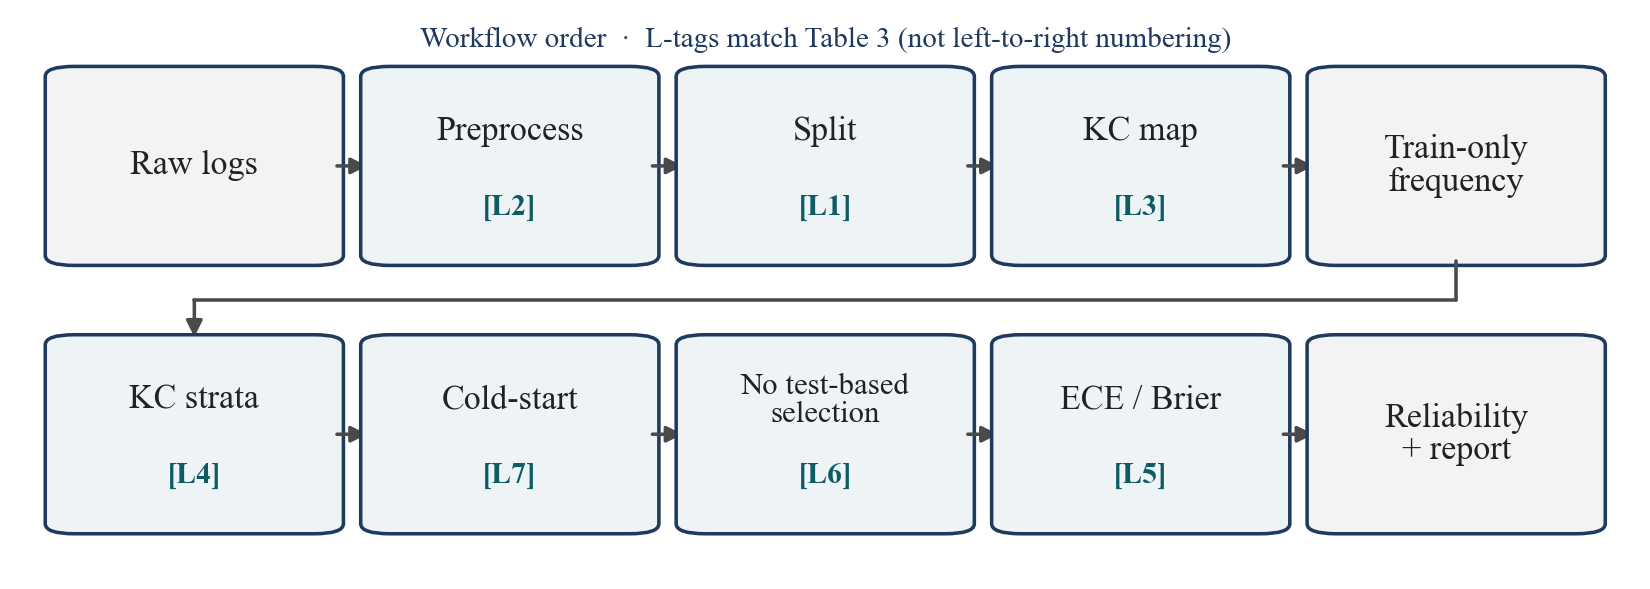
\includegraphics[width=\textwidth]{figures/fig1.png}
\par\vspace{0.45em}
{\fontsize{8}{10}\selectfont Fig. 1. Reproducible sparse-concept and calibration diagnostic pipeline. Tags L1--L7 match Table 3. L3 --- KC map / Q-matrix: static platform-provided mapping (the figure box reads KC map). L5: no test-fit map; L6: no test-based model selection; L7: f\_train=0.\par}
\end{minipage}
\vspace{0.55em}
\noindent\begin{minipage}{\textwidth}
\centering
{\fontsize{8}{9.5}\selectfont Table 3. Seven-channel leakage checklist for the evaluation pipeline (learner-based fold 0). PASS means the listed decision was applied without using test data for model or hyperparameter selection. L6 is no test-based model selection: a fixed training schedule / final checkpoint; test data are used only for reporting. Compact learner-based fold-0 slice of Table A5 (same characters, including occupancy flags). L3 --- KC map / Q-matrix: static platform-provided mapping. For Junyi, ucid is an operational content/exercise identifier, not a manually curated skill tag.\par}
\vspace{0.35em}
\begin{adjustbox}{max width=\textwidth}
{\small
\begin{tabular}{@{}lllll@{}}
\toprule
Channel & Decision & Assist. & Junyi & XES3G5M \\
\midrule
L1 Split & Learner-disjoint users & PASS & PASS & PASS \\
L2 Preprocess & Train-only transforms & PASS & PASS & PASS \\
L3 --- KC map / Q-matrix & Static platform-provided mapping & PASS & PASS & PASS \\
L4 Bucket & f\_train cuts only & PASS & PASS (EMPTY) & PASS \\
L5 Calibration & No test-fit map & PASS & PASS & PASS \\
L6 Selection & No test-based model selection (fixed schedule / final checkpoint) & PASS & PASS & PASS \\
L7 Cold-start & f\_train=0 documented & PASS (EMPTY) & PASS (EMPTY) & PASS (I) \\
\bottomrule
\end{tabular}}
\end{adjustbox}
\end{minipage}
\vspace{0.55em}
\begin{multicols}{2}


Under the learner-disjoint split every test learner is unseen at training time, so in our implementation the IRT column reduces by construction to a global training base-rate predictor and its AUC is exactly 0.5000; item difficulty $\beta$ is estimated during training but is not used at prediction time for unseen learners. We report it as a base-rate reference. The result is specific to this implementation, not to item-response theory in general.

\subsection*{D. Train-only frequency strata}

For each fold, KC frequency ftrain is counted on the training file only. Buckets: strict cold-start (f=0), very sparse (0$<$f$<$20), sparse (20$\leq$f$<$100), medium (100$\leq$f$<$500), dense (f$\geq$500). Fig. 2 (top) shows the number of KCs in each stratum. Training-interaction volume is shown separately in the bottom row from summed ftrain, not inferred from KC counts. The protocol then applies four steps on each fold: (1) assign those train-only strata, including f=0; (2) flag sample support as Reliable, Limited, or Insufficient (Section III.E); (3) report calibration by stratum with those flags; (4) optionally apply one locked threshold and report the false-advance rate as a probe (Section III.E--H).

\subsection*{E. Reliability flags}

Occupancy flags follow test-event count N: Reliable (R) N$\geq$1000; Limited (L) 100$\leq$N$<$1000; Insufficient (I) N$<$100. We call R, L, and I descriptive sample-support flags. They are not inferential guarantees, confidence intervals, or hypothesis tests. Substantive stratum-level interpretations require at least Limited support; Insufficient cells are descriptive only. Very-sparse ASSISTments cells are Insufficient and descriptive only.


\end{multicols}
\noindent\begin{minipage}{\textwidth}
\centering
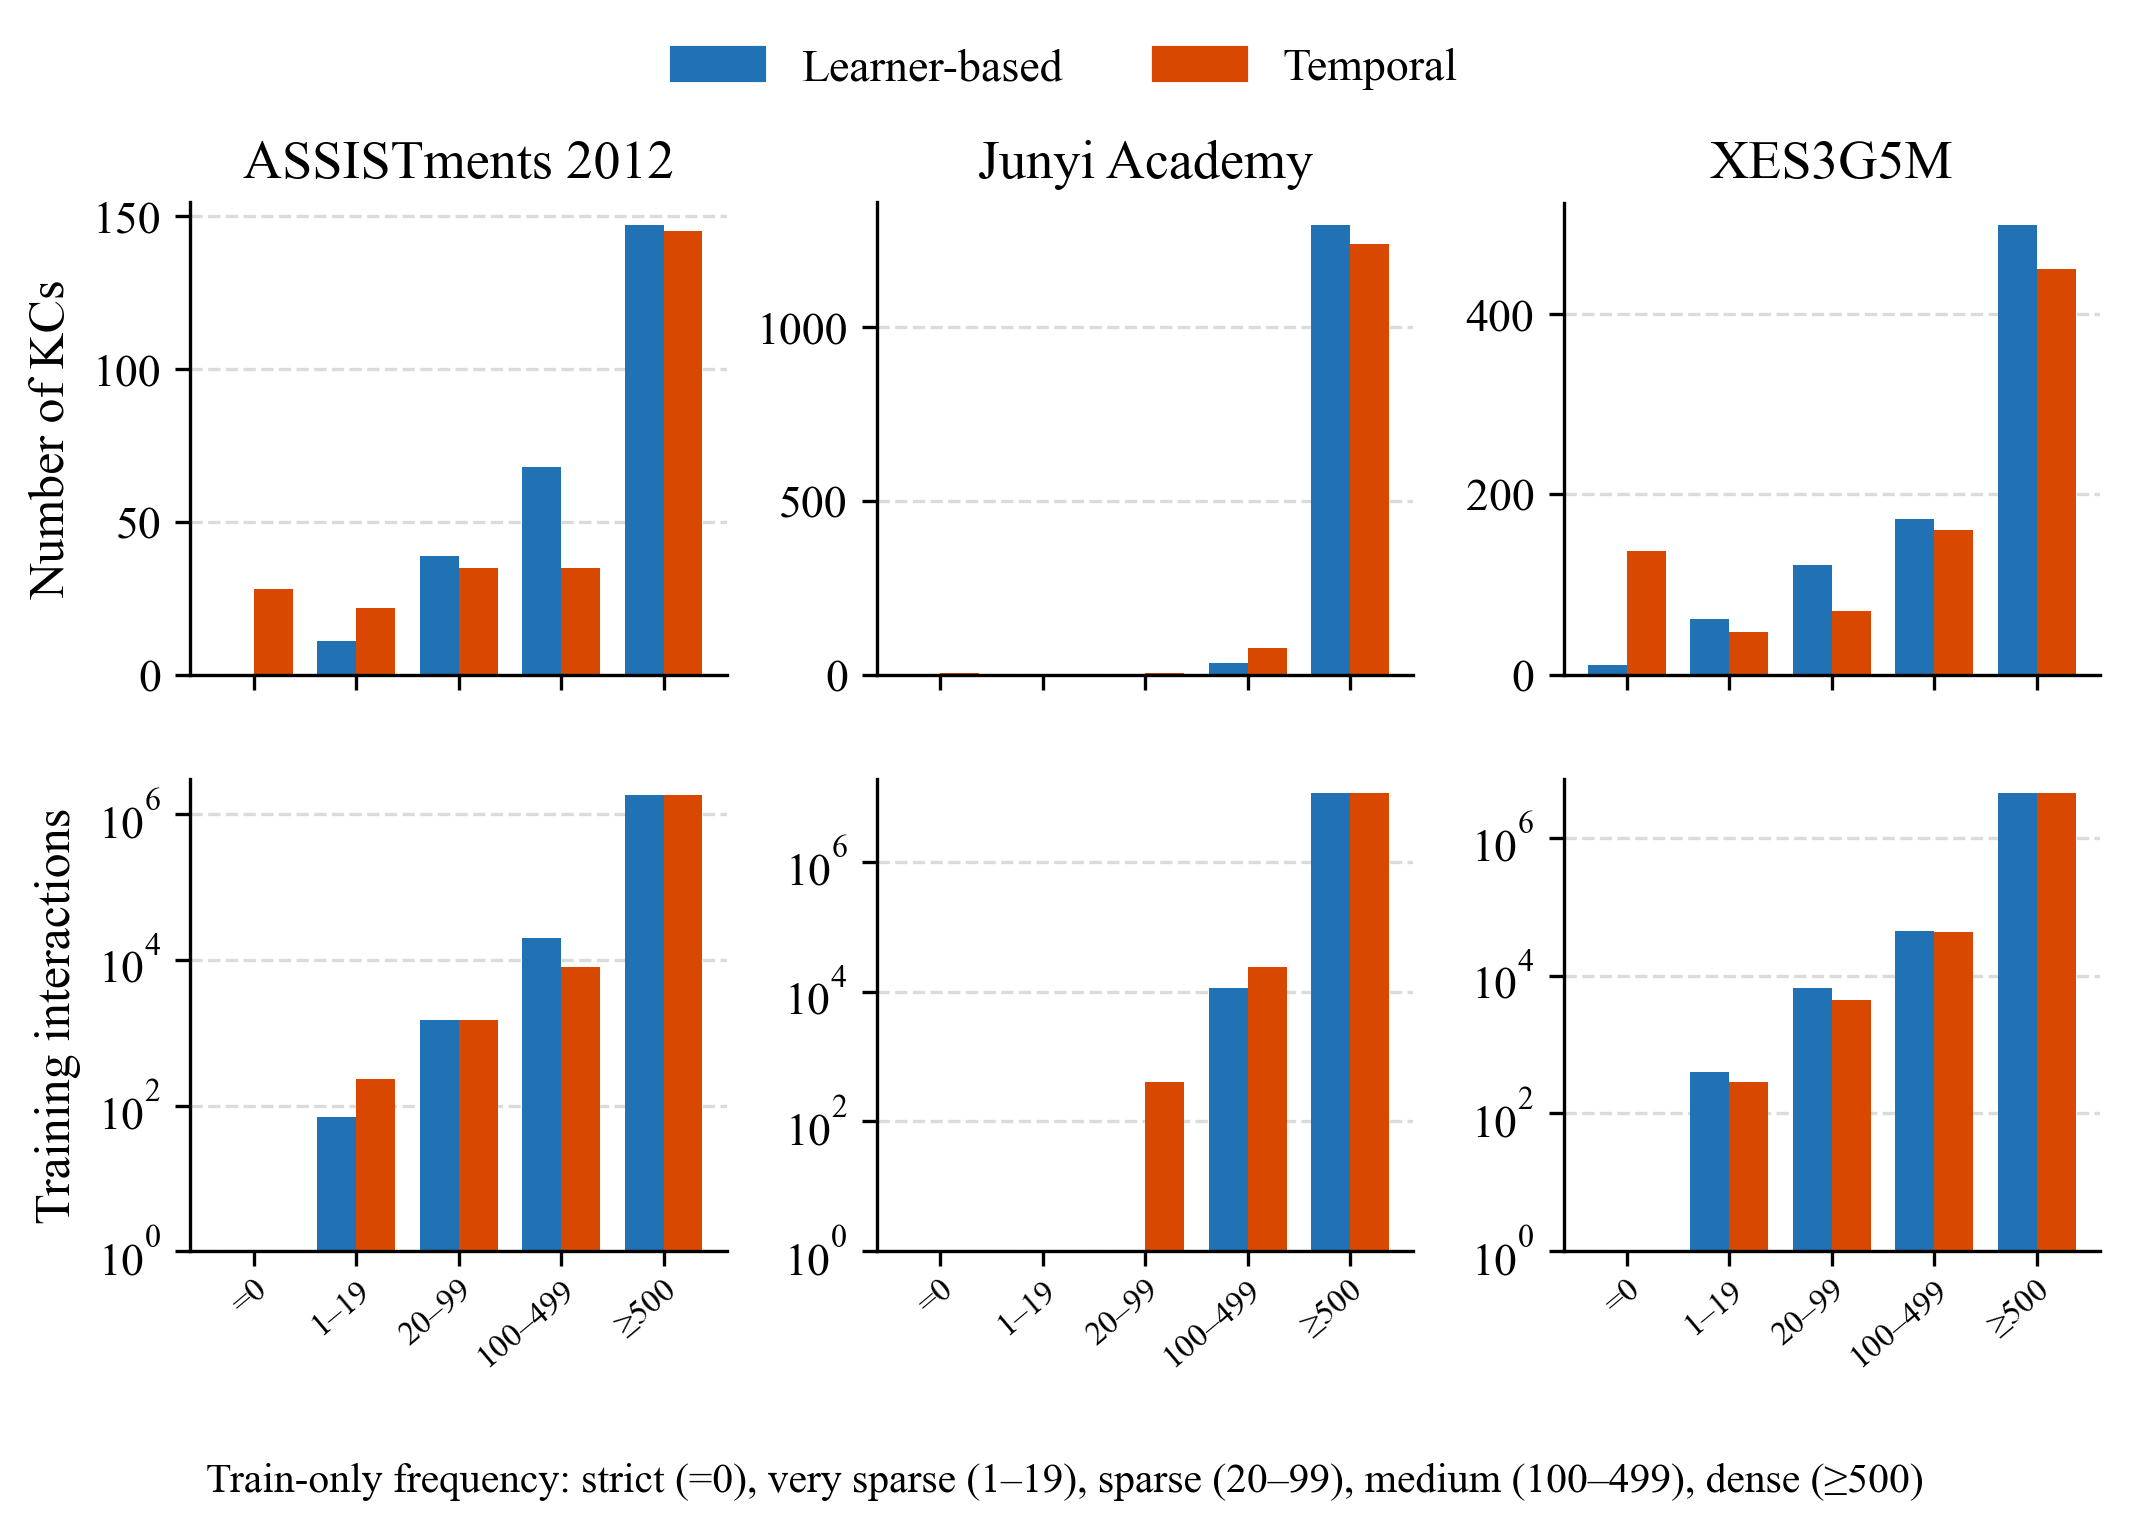
\includegraphics[width=\textwidth]{figures/fig2.png}
\par\vspace{0.45em}
{\fontsize{8}{10}\selectfont Fig. 2. Distribution of KCs across train-only frequency strata under learner-based and temporal splits. Bottom: verified training-interaction counts (sum of train-only ftrain on fold 0); volume is not inferred from KC counts. Bottom y-axis is logarithmic.\par}
\end{minipage}
\vspace{0.55em}
\begin{multicols}{2}


\subsection*{F. Calibration}

Let $y\in\{0,1\}$ be next-response correctness and $p\in[0,1]$ the predicted probability. With M=15 equal-width bins, expected calibration error (ECE) is

\begin{equation}
\mathrm{ECE}=\sum_{m}(n_{m}/N)\left|\mathrm{acc}_{m}-\mathrm{conf}_{m}\right|
\end{equation}

The Brier score is (1/N) $\Sigma$\_i (p\_i $-$ y\_i)$^2$. We use the binned Murphy decomposition Brier = UNC $-$ RES + REL [18], with UNC = $\bar{y}$(1$-$$\bar{y}$), REL = (1/N) $\Sigma$\_m n\_m (conf\_m $-$ acc\_m)$^2$, and RES = (1/N) $\Sigma$\_m n\_m (acc\_m $-$ $\bar{y}$)$^2$. Because probabilities are binned, the three components are an empirical approximation and need not sum exactly to the directly computed Brier score. Lower ECE is better calibration; it is not a substitute for AUC.

\subsection*{G. Difficulty coupling}

For each KC c we define a training-only difficulty proxy difficulty(c) = 1 $-$ mean\_train\_correctness(c). The mean is taken on the training file only. This is an observational proxy for how often c is answered incorrectly in training; it is not a latent IRT difficulty parameter. The reported Spearman association is $\rho$(log(1+f$_{train}$), difficulty), computed on training-fold KC summaries. The same file yields item support (distinct items per KC), learner exposure (distinct learners per KC), and a curriculum-position proxy (median normalized sequence position). Results report between-KC associations and a within-KC sparsification check; neither identifies a causal frequency effect.

\subsection*{H. Simulated decision-error probe (not the primary claim)}

For a locked global threshold $\tau$, the system advances (skips remediation) if p$\geq$$\tau$ and triggers remediation otherwise. Sparse events never receive their own tuned $\tau$ in the display rule: Tables A2--A3 use one locked global $\tau$=0.7. On ASSISTments 2012 fold 0, T-KT $\Delta$FAR stays positive at every locked grid point $\tau\in\{0.5, 0.6, 0.7, 0.8\}$ (Table A6); the grid is not a search over sparse error. A separate counterfactual analysis in the accompanying artifact evaluates the same frozen predictions under a Reliable-only advance rule and under a mixed-threshold rule (sparse $\tau$=0.8, otherwise $\tau$=0.7); neither is a trained or displayed rule.

Let $A=\{p\geq\tau\}$. The false-advance rate (FAR) is P(y=0 | p$\geq$$\tau$): among responses for which the simulated system would advance the learner, the proportion whose observed next response is incorrect. Equivalently, FAR = 1 $-$ precision among events with p$\geq$$\tau$. This is not a measurement of latent mastery. It is a next-response decision-error proxy under a simulated threshold gate. The corresponding false-positive rate is FPR = P(p$\geq$$\tau$ | y=0). Expected FAR under the model probabilities is E[1$-$p | p$\geq$$\tau$]. Excess FAR = FAR $-$ E[1$-$p | p$\geq$$\tau$]. $\Delta$FAR = FAR\_sparse $-$ FAR\_dense. FAR is a proportion of Nadvance = count(p$\geq$$\tau$) events, not of N\_total; FPR is a proportion of Nincorrect = count(y=0). N\_total alone does not imply the precision of FAR. Where prediction-level exports exist, 95\% intervals use the KC-clustered percentile bootstrap already used for this gate (B=2000, resample KCs within sparse and within dense). Positive $\Delta$FAR means sparse advance decisions are less reliable than dense advance decisions. This is a simulated decision error, not an instructional randomized controlled trial (RCT).

\section*{\MakeUppercase{IV. RESULTS}}

\subsection*{A. Aggregate discrimination}

\looseness=2 Table 4 reports overall learner-based AUC and accuracy (ACC), mean$\pm$sd over four unique partitions. This subsection is discrimination, not calibration. DKT is slightly above T-KT on all three datasets (ASSISTments DKT 0.6979$\pm$0.0014 versus T-KT 0.6837$\pm$0.0025). Official SimpleKT [4] on the same ASSISTments partitions reaches 0.7700$\pm$0.0013 (ACC 0.7522$\pm$0.0014); T-KT is not that checkpoint. pyKT [5] uses standardized sequence-level preprocessing and split conventions that differ from the learner-disjoint protocol used here; absolute AUC values are therefore not directly comparable across the two evaluation settings. We do not attempt to match leaderboard numbers: one preprocessing and evaluation pipeline is held fixed across strata so that dense and sparse cells are comparable to each other. Stratum-level AUC and ACC for IRT, DKT, and T-KT are in the accompanying artifact. Under the learner-disjoint split every test learner is unseen, so the IRT column is a global training base-rate predictor by construction (AUC exactly 0.5000); $\beta$ is estimated in training but unused at prediction for unseen learners. It is a base-rate reference, not a ranking competitor.


\end{multicols}
\noindent\begin{minipage}{\textwidth}
\centering
{\fontsize{8}{9.5}\selectfont Table 4. Overall learner-based area under the ROC curve (AUC) and accuracy (ACC) (mean$\pm$sd over four unique partitions). IRT is a base-rate reference (AUC=0.5000 by construction under the learner-disjoint split), not a ranking competitor. Official SimpleKT [4] is reported on ASSISTments only.\par}
\vspace{0.35em}
\begin{adjustbox}{max width=\textwidth}
{\small
\begin{tabular}{@{}llll@{}}
\toprule
Dataset & Model & AUC & ACC \\
\midrule
ASSISTments 2012 & IRT (base-rate) & 0.5000 & 0.6973$\pm$0.0004 \\
ASSISTments 2012 & DKT & 0.6979$\pm$0.0014 & 0.7182$\pm$0.0014 \\
ASSISTments 2012 & T-KT & 0.6837$\pm$0.0025 & 0.6996$\pm$0.0032 \\
ASSISTments 2012 & SimpleKT & 0.7700$\pm$0.0013 & 0.7522$\pm$0.0014 \\
Junyi Academy & IRT (base-rate) & 0.5000 & 0.7053$\pm$0.0018 \\
Junyi Academy & DKT & 0.7320$\pm$0.0009 & 0.7343$\pm$0.0015 \\
Junyi Academy & T-KT & 0.7220$\pm$0.0035 & 0.7267$\pm$0.0035 \\
XES3G5M & IRT (base-rate) & 0.5000 & 0.7961$\pm$0.0031 \\
XES3G5M & DKT & 0.8180$\pm$0.0009 & 0.8321$\pm$0.0015 \\
XES3G5M & T-KT & 0.7536$\pm$0.0010 & 0.8057$\pm$0.0029 \\
\bottomrule
\end{tabular}}
\end{adjustbox}
\end{minipage}
\vspace{0.55em}
\begin{multicols}{2}


On XES3G5M, sparse-stratum AUC is higher than dense-stratum AUC (DKT 0.858 versus 0.818; T-KT 0.847 versus 0.752; Reliable occupancy). Lower training frequency is therefore not a universal ranking failure. Junyi's learner-based sparse bucket is empty under the pre-specified cuts---a protocol outcome, not a missing cell and not a zero-ECE claim.

\subsection*{B. Calibration across frequency strata}

Table 5 reports event-level ECE, not AUC. On ASSISTments 2012, T-KT ECE increases from 0.1136$\pm$0.0066 (dense, Reliable, N=523,971) to 0.1541$\pm$0.0051 (medium) to 0.2280$\pm$0.0197 (sparse, Limited, N=415). That sparse cell is Limited support, not a high-N finding. Because binned ECE is sensitive to finite sample size and bin occupancy, Limited-support sparse ECE is interpreted as an occupancy-aware diagnostic warning rather than an inferential proof of worse calibration. Official SimpleKT [4] on those partitions has ECE 0.0203$\pm$0.0035 dense and 0.0884$\pm$0.0187 sparse (Limited, N=415); the rise remains, and the T-KT cells stay locked. That official SimpleKT result is an external ASSISTments check of whether the observed dense-to-sparse ECE direction is unique to the local T-KT reference; it is not generalized to Junyi or XES3G5M. DKT moves in the same direction on this dataset (dense 0.0602$\pm$0.0022 versus sparse 0.2333$\pm$0.0084). The ECE rise is corroborated by higher Brier reliability error and Brier score on ASSISTments (Table 6). IRT dense ECE is 0.0031$\pm$0.0006, but resolution is zero (Table A4a): a near-constant predictor can look calibrated while providing no ranking information. Frozen ASSISTments IRT prediction files on the four unique learner partitions give mean(y)=0.6996 dense and 0.6365 sparse, with a near-constant IRT score mean(p)$\approx$0.6962. The pooled frozen IRT export gives those mean(y) values, whereas Table A4a reports the mean of partition-level Murphy components, so pooled mean(y)(1$-$mean(y)) need not equal the reported mean UNC exactly; the IRT export also uses a slightly different valid-event subset (sparse N mean 407) from the Table 5 ECE cell (N=415). Table A4a IRT ECE (0.0031$\pm$0.0006 dense; 0.0777$\pm$0.0555 sparse) is a constant-predictor base-rate reference, not a mathematical lower bound. On the same frequency-defined sparse stratum, T-KT and DKT show numerically larger ECE than that reference; because the valid-event subsets are not identical and binned ECE is sensitive to sample size and bin occupancy, this comparison is descriptive only. The IRT cell combines low ECE with zero resolution, which illustrates why calibration must be read together with discrimination and resolution; it is not evidence that IRT is well calibrated as a ranking model. The constant-predictor reference is used only to contextualize stratum-level base-rate shift; it is not treated as a lower bound on attainable calibration error, nor as a calibrated competitive model.

Calibration does not universally worsen. On Junyi Academy the learner-based sparse bucket is empty. Only dense and medium exist. T-KT ECE rises from 0.0817$\pm$0.0070 to 0.1136$\pm$0.0155 (same scored N as DKT/IRT after aligning T-KT exports to official learner partitions; Fig. 3). On XES3G5M, T-KT ECE does not show the same adverse dense-to-sparse gradient as ASSISTments. The observed values are 0.1176, 0.1129, and 0.1254. They differ by a small amount relative to the ASSISTments contrast, despite Reliable sparse occupancy (N=1,969). T-KT Brier is not worse on sparse than dense (0.149 vs 0.156). That difference is interpreted descriptively. DKT on the same XES partitions is not a counter-pattern: ECE, Brier, and REL all rise from dense to sparse (Table A4b). Occupancy is still reported with that pattern. It is not a flat FPR.


\end{multicols}
\noindent\begin{minipage}{\textwidth}
\centering
{\fontsize{8}{9.5}\selectfont Table 5. T-KT and official SimpleKT [4] (ASSISTments only) event-level expected calibration error (ECE) by train-only frequency stratum. N is the mean test-event count across four unique learner partitions after prediction export and stratum assignment, not a fold-0 processed-event count (Table 1). Stratum N values are not expected to match or sum exactly to Table 1. Flags: Reliable (R) N$\geq$1000; Limited (L) 100$\leq$N$<$1000. Junyi sparse is empty. Junyi medium T-KT ECE 0.1136 is not the ASSISTments dense T-KT cell. Junyi T-KT averages two initializations on official fold 0 before the equal-weight four-partition mean used for DKT and IRT.\par}
\vspace{0.35em}
\begin{adjustbox}{max width=\textwidth}
{\small
\begin{tabular}{@{}lllll@{}}
\toprule
Dataset & Stratum & N & Flag & ECE \\
\midrule
ASSISTments 2012 & dense & 523,971 & R & 0.1136$\pm$0.0066 \\
ASSISTments 2012 & medium & 5,963 & R & 0.1541$\pm$0.0051 \\
ASSISTments 2012 & sparse & 415 & L & 0.2280$\pm$0.0197 \\
Assist. SimpleKT & dense & 523,971 & R & 0.0203$\pm$0.0035 \\
Assist. SimpleKT & medium & 5,963 & R & 0.0262$\pm$0.0025 \\
Assist. SimpleKT & sparse & 415 & L & 0.0884$\pm$0.0187 \\
Junyi Academy & dense & 3,226,541 & R & 0.0817$\pm$0.0070 \\
Junyi Academy & medium & 3,706 & R & 0.1136$\pm$0.0155 \\
XES3G5M & dense & 1,269,345 & R & 0.1176$\pm$0.0014 \\
XES3G5M & medium & 12,889 & R & 0.1129$\pm$0.0061 \\
XES3G5M & sparse & 1,969 & R & 0.1254$\pm$0.0047 \\
\bottomrule
\end{tabular}}
\end{adjustbox}
\end{minipage}
\vspace{0.55em}
\noindent\begin{minipage}{\textwidth}
\centering
{\fontsize{8}{9.5}\selectfont Table 6. Four-partition Brier score and Murphy decomposition (UNC $-$ RES + REL) by train-only stratum. N is the mean test-event count. Junyi sparse is empty. Junyi T-KT N matches DKT/IRT after alignment to official learner partitions. Full Brier, UNC, REL, and RES grids, including XES3G5M, are in Tables A4a--A4b.\par}
\vspace{0.35em}
\begin{adjustbox}{max width=\textwidth}
{\small
\begin{tabular}{@{}lllllllll@{}}
\toprule
Dataset & Model & Stratum & N & ECE & Brier & UNC & REL & RES \\
\midrule
ASSISTments & DKT & dense & 523,971 & 0.0602 & 0.1931 & 0.2103 & 0.0053 & 0.0223 \\
ASSISTments & DKT & sparse & 415 & 0.2333 & 0.2502 & 0.2337 & 0.0624 & 0.0451 \\
ASSISTments & T-KT & dense & 523,971 & 0.1136 & 0.2116 & 0.2103 & 0.0201 & 0.0186 \\
ASSISTments & T-KT & sparse & 415 & 0.2280 & 0.2525 & 0.2337 & 0.0594 & 0.0392 \\
Junyi & DKT & dense & 3,226,541 & 0.0389 & 0.1804 & 0.2078 & 0.0022 & 0.0294 \\
Junyi & DKT & medium & 3,706 & 0.2513 & 0.3077 & 0.2432 & 0.0741 & 0.0091 \\
Junyi & T-KT & dense & 3,226,541 & 0.0817 & 0.1892 & 0.2078 & 0.0091 & 0.0275 \\
Junyi & T-KT & medium & 3,706 & 0.1136 & 0.2347 & 0.2432 & 0.0163 & 0.0251 \\
\bottomrule
\end{tabular}}
\end{adjustbox}
\end{minipage}
\vspace{0.55em}
\begin{multicols}{2}


\subsection*{C. Cold-start concept feasibility}

Strict cold-start is freq\_train(c)=0. The next Table 7 slice is the protocol very-sparse bucket (0$<$freq\_train(c)$<$20). Table 7 reports feasibility, not a production claim. On ASSISTments 2012 the strict bin has a four-partition mean of about four test events (Insufficient; Table 7), not the fold-0 count, and the very-sparse bin about 17 events (Insufficient), so ECE/AUC on those slices are descriptive only. Junyi's learner-based operational identifier (ucid) yields no estimable sparse or strict-cold-start stratum. XES3G5M very-sparse support is larger (N$\approx$114) but still not a high-N finding. Where the strict slice is too small, the protocol records the empty or Insufficient bucket instead of borrowing a recommender user/item cold-start definition.


\end{multicols}
\noindent\begin{minipage}{\textwidth}
\centering
{\fontsize{8}{9.5}\selectfont Table 7. Cold-start concept feasibility (four-partition means). Strict: f\_train=0. Very-sparse: 0$<$f\_train$<$20. L/I are occupancy flags on test-event count N. I = Insufficient (N$<$100). Insufficient cells (N$<$100) report descr.; ECE is not a supported finding on those slices. Not a recommender user/item split. XES3G5M very-sparse uses the same masked four-partition series as Table 5 (N=114).\par}
\vspace{0.35em}
\begin{adjustbox}{max width=\textwidth}
{\small
\begin{tabular}{@{}llllll@{}}
\toprule
Dataset & Slice & Mean N & Flag & T-KT ECE & DKT ECE \\
\midrule
ASSISTments & strict f=0 & 4 & I & descr. & descr. \\
ASSISTments & very-sparse & 17 & I & descr. & descr. \\
Junyi & strict / sparse & 0 & empty & --- & --- \\
XES3G5M & very-sparse & 114 & L & 0.184 & 0.173 \\
\bottomrule
\end{tabular}}
\end{adjustbox}
\end{minipage}
\vspace{0.55em}
\begin{multicols}{2}


\subsection*{D. Diagnostic conditions and threshold sensitivity}

If a learning platform uses KT probabilities only to sort students, Table 4 may suffice. If it uses p to skip practice or declare mastery, Table 4 is an insufficient evaluation summary. The ASSISTments T-KT cell is an illustrative case: aggregate discrimination that does not reveal the sparse-stratum calibration pattern, Limited-but-estimable sparse occupancy (about 19\% of KCs fall below the sparse threshold on fold 0), a monotonic ECE rise, and a gate that yields a higher error rate among sparse advance decisions. The XES3G5M cell is the contrasting T-KT ECE case: plenty of low-frequency tail mass (f\_train$<$100) and Reliable occupancy, yet T-KT ECE does not show the same adverse dense-to-sparse gradient as ASSISTments (DKT ECE/Brier/REL do; Table A4b). Junyi shows that the protocol can refuse a sparse claim when the bucket is empty.

The following checks are secondary evidence for why and when a sparse-calibration contrast is estimable; they do not replace the per-stratum ECE and Brier results. Table A1 checks the same ASSISTments T-KT dense-to-sparse ECE rise under two alternative train-only cut grids; the sign does not flip. Across the three cut grids, $\Delta$ECE decreases monotonically as the sparse stratum grows (T-KT: 0.1260 at N = 303, 0.1144 at N = 415, 0.1049 at N = 685; DKT: 0.1853, 0.1731, 0.1487). Two explanations are consistent with this pattern and are not separated by the present design: binned ECE is upward-biased at small bin occupancy [26], [27], and a wider cut grid also admits less sparse KCs into the bucket. We therefore read Table A1 as evidence that the sign of the contrast is stable, not as evidence about its magnitude. Table 8 separates two questions. E1--E2 determine whether a sparse contrast can be estimated under the protocol thresholds; E3 and other structural descriptors help characterize the direction of the observed pattern. E1 is a non-empty low-frequency tail under the split actually used; E2 is enough sparse test events for at least a Limited-flag ECE. E3 (frequency--difficulty coupling) is not treated as necessary or sufficient for an adverse gradient. Junyi fails E1--E2. ASSISTments and XES3G5M both meet E1--E2, yet only ASSISTments shows a dense-to-sparse T-KT ECE rise.


\end{multicols}
\noindent\begin{minipage}{\textwidth}
\centering
{\fontsize{8}{9.5}\selectfont Table 8. Empirical conditions associated with the availability and direction of sparse-calibration contrasts on the three evaluated datasets. Low-frequency tail mass: share of KCs with train-only frequency ftrain$<$100. E3 is not necessary or sufficient for an adverse gradient.\par}
\vspace{0.35em}
\begin{adjustbox}{max width=\textwidth}
{\small
\begin{tabular}{@{}llll@{}}
\toprule
Condition & ASSISTments & Junyi & XES3G5M \\
\midrule
\multicolumn{4}{l}{A. Estimability} \\
Low-frequency tail mass (E1) & 18.9\% of KCs & 0\% & 21.5\% of KCs \\
Sparse test support (E2) & 415 (L) & empty & 1,969 (R) \\
\multicolumn{4}{l}{B. Observed pattern/context} \\
Difficulty coupling (E3) & $\rho$=$-$0.227 (sparse harder) & $\rho$=$-$0.416 & $\rho$=+0.110 (weak, inverted) \\
Item support & median 44.5 (dense 205 vs sparse 1) & median 18 (IQR 5) & median 3 (dense 9 vs sparse 1) \\
Curriculum-position coupling & $\rho$=$-$0.308 & $\rho$=$-$0.324 & $\rho$=$-$0.126 \\
Observed T-KT ECE & 0.114 to 0.228 & dense to medium only & 0.1176 / 0.1129 / 0.1254 (descr.) \\
\bottomrule
\end{tabular}}
\end{adjustbox}
\end{minipage}
\vspace{0.55em}
\noindent\begin{minipage}{\textwidth}
\centering
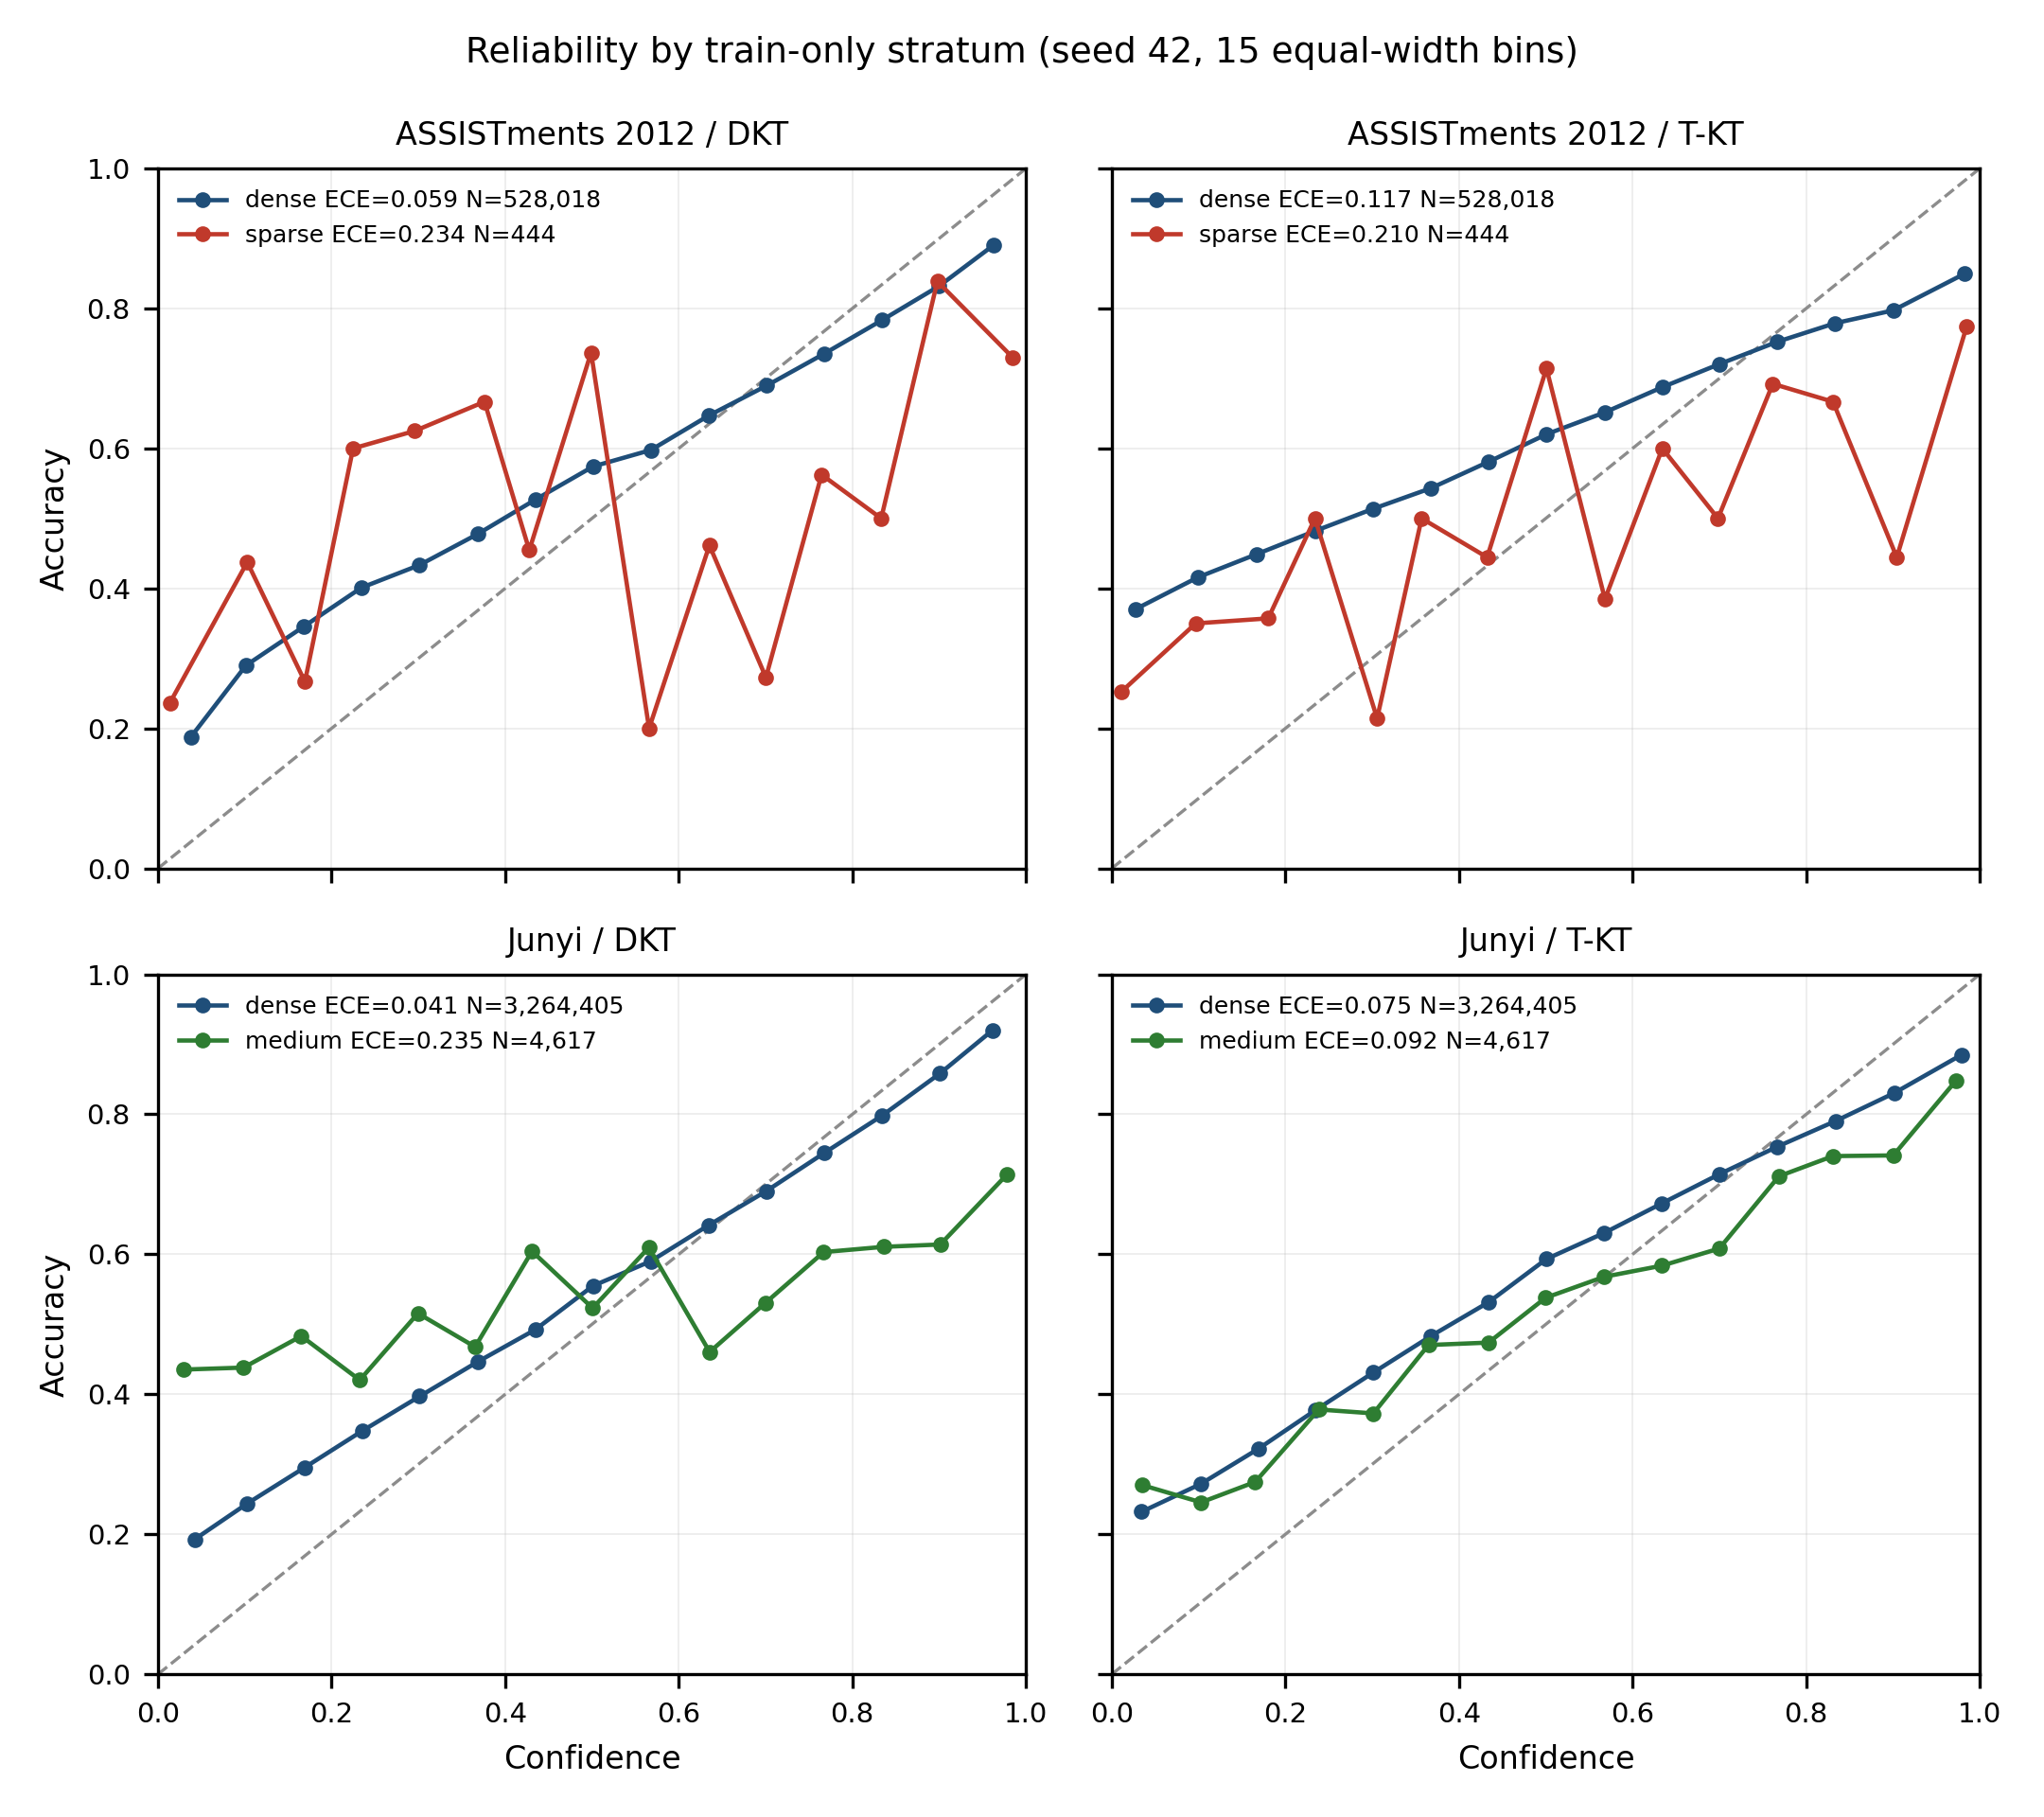
\includegraphics[width=\textwidth]{figures/fig3.png}
\par\vspace{0.45em}
{\fontsize{8}{10}\selectfont Fig. 3. Reliability diagrams (15 equal-width bins; seed 42 only) are visual diagnostics. Tables 5 and 6 report four-partition means. Rows: ASSISTments 2012 and Junyi Academy. Columns: DKT and T-KT. ASSISTments panels show dense vs sparse; Junyi panels show dense vs medium (learner-based sparse is empty). Not a classroom trial.\par}
\end{minipage}
\vspace{0.55em}
\begin{multicols}{2}


\subsection*{E. Secondary explanatory analysis}

Learner exposure (distinct training learners per KC) enters the regressions below; it is not an E1--E2 estimability criterion. The regression and sparsification checks are not causal claims.

A test-event-weighted KC-level regression of T-KT ECE on those five training-only covariates is a between-KC association: it compares different concepts. ASSISTments (478 KC-fold rows; 261 unique KCs) and Junyi (2,645 KC-fold rows; 1,326 unique KCs) use cluster-robust standard errors at kc\_id; XES3G5M is 829 unique KCs in the masked weighted fit. Standardized log(1+ftrain) coefficients are $-$0.068 [$-$0.086, $-$0.050] on ASSISTments, $-$0.014 [$-$0.018, $-$0.010] on Junyi, and $-$0.028 [$-$0.042, $-$0.014] on XES3G5M in the weighted fit. Difficulty is independently associated on all three datasets. Learner exposure is independently associated on ASSISTments (+0.016 [0.004, 0.027]) and on XES3G5M (+0.013 [+0.005, +0.021]). These signs do not test a frequency dose on a fixed KC.

Controlled sparsification does not reproduce a universal monotonic frequency effect: of 18 dataset--model--reduction cells (three datasets $\times$ DKT/T-KT $\times\{500, 100, 50\}$ training rows; 30 originally dense KCs each; seed 42), nine of 18 cells have 95\% KC-bootstrap percentile intervals (B=10,000) entirely above 0, four entirely below 0, and five that include 0 (frozen grid in the accompanying artifact).

The three analyses target different estimands: stratum ECE is an event-weighted coarse-bucket contrast, the regression estimates an adjusted between-KC association, and controlled sparsification evaluates an artificial within-KC reduction of training evidence. Their signs and magnitudes therefore need not coincide.

\subsection*{F. Secondary decision-error probe}

\looseness=2 A locked gate at $\tau$=0.7 is a simulated next-response decision-error probe, not RQ3. On ASSISTments 2012, T-KT FAR is 0.196 on dense KCs and 0.268 on sparse KCs ($\Delta$FAR = +0.072; seed 42; KC-clustered percentile bootstrap 95\% CI [0.006, 0.138], B = 2000), and $\Delta$FAR is positive in 4/4 unique learner partitions (partition-level mean 0.056). For DKT the same probe is positive in only 3 of 4 unique partitions (Table A3; five-run count 3/5 is a different unit), so the stratum difference in gate error is not uniform across backbones; the lower confidence bound for T-KT is close to zero, and we therefore report the direction of $\Delta$FAR, not its robustness. On XES3G5M the same T-KT probe points the other way: $\Delta$FAR is negative in all 4/4 unique learner partitions (partition-level mean $\Delta$FAR = $-$0.019; five-run mean $-$0.017; sparse N mean 1,957 (five-run gate; not the four-partition ECE N=1,969); accompanying artifact). ASSISTments FAR denominators and partition-level summaries are reported in Tables A2--A3; the occupancy-policy counterfactual remains in the accompanying artifact; the $\tau$-grid is Table A6.

\columnbreak
\section*{\MakeUppercase{V. DISCUSSION}}

\subsection*{A. Main empirical findings}

Two empirical regularities, not laws, structure the results. First, training frequency is not a universal predictor of AUC failure: on XES3G5M, sparse-stratum AUC is higher than dense-stratum AUC for DKT and T-KT (Reliable occupancy), and Junyi's learner-based sparse bucket is empty (exercise-level operational identifier, ucid) rather than a ranking collapse. Second, the observed sparse-stratum calibration pattern is dataset- and model-dependent. ASSISTments 2012 T-KT ECE is associated with a dense-to-sparse rise under Limited sparse support (Table 5, N=415); XES3G5M T-KT ECE does not show the same adverse dense-to-sparse gradient as ASSISTments (0.1176 / 0.1129 / 0.1254; Section IV.B) despite Reliable sparse occupancy, while XES DKT ECE/Brier/REL worsen. Calibration is not guaranteed to worsen as frequency falls. As a secondary operational probe, a locked next-response gate can differ by frequency stratum: ASSISTments T-KT $\Delta$FAR is positive in 4/4 unique partitions (direction only; seed-42 95\% CI [0.006, 0.138]), DKT is positive in only 3/4 unique partitions (Table A3), and the XES3G5M T-KT probe points the other way, with $\Delta$FAR negative in all 4/4 unique learner partitions (partition-level mean $-$0.019; five-run mean $-$0.017; accompanying artifact; ASSISTments denominators in Tables A2--A3).

\subsection*{B. Practical implications for educational technology}

Educational-technology gates that skip, remediate, or advance practice consume a predicted probability, not a population AUC. A ranking win can therefore hide miscalibration on rarely practiced KCs. This subsection is a pre-deployment evaluation checklist for that probability-to-decision chain, not a recommended production threshold. Four checks precede any operational reading of a single global threshold. (1) Occupancy: inspect train-only KC-frequency occupancy on the training fold actually used, and report empty or low-support strata. (2) Calibration: evaluate ECE and Brier/reliability by stratum rather than relying only on population AUC. (3) Threshold decision error: if a fixed probability gate is evaluated, report FAR and FPR with their denominators. FAR = P(y=0 | p$\geq$$\tau$) and equals 1 $-$ precision among advance decisions; FPR = P(p$\geq$$\tau$ | y=0). (4) Leakage/evaluation hygiene: before operational interpretation, verify the relevant L1--L7 decisions, especially train-only stratum assignment, no test-fitted calibration map, no test-based model selection, and a cold-start definition from training frequency. Reliable/Limited/Insufficient flags remain descriptive sample-support labels, not inferential guarantees. This study does not apply temperature scaling [16] or Platt scaling [28]. A population AUC win is not by itself evidence that probabilities are reliable on the tail.

\subsection*{C. Why datasets differ}

\looseness=2 The three logs differ on E1--E2 estimability and on structural context (Table 8). Junyi's learner-based sparse bucket is empty because the operational field is ucid (an exercise-level identifier, not a skill tag), so the protocol can refuse a sparse claim when the unit is finer than a skill. Junyi is therefore interpreted primarily as a granularity-and-estimability case rather than direct evidence about pedagogical KC sparsity. ASSISTments and XES3G5M both have a non-empty sparse tail and at least Limited test support, yet T-KT ECE rises on ASSISTments and does not show the same adverse dense-to-sparse gradient on XES3G5M. Frequency--difficulty coupling, item support, and curriculum-position coupling are reported as context, not as necessary or sufficient conditions for that direction. Within-KC sparsification (reported in the accompanying artifact) does not reproduce the observational ASSISTments T-KT ECE gradient. These are associations on these datasets. Untested explanations---curriculum hierarchy, tagging granularity, ceiling effects, and item semantics---are hypotheses unless experimentally isolated, which this study does not do.

\subsection*{D. Limitations}

\looseness=3 Next-response correctness is not latent mastery: y=0 is an incorrect next attempt, not a latent-skill diagnosis. The threshold gate is the simulated probe defined in Section III.H. There is no classroom RCT. We do not train graph, contrastive, or self-supervised KT models. BKT is not a scored baseline because pyBKT 1.4.1 produced a degenerate fit on the tested ASSISTments seed-42 configuration (reported in the accompanying artifact). IRT is the classical reference. T-KT is the local reference in Section III.C. Official SimpleKT remains the external ASSISTments check reported there. Temporal evaluation uses a single corrected cutoff (seed 42). Seeds 2025 and 2026 share a split. R/L/I are descriptive support flags. ECE depends on binning. We do not report size-matched or cluster-bootstrap confidence intervals for primary stratum $\Delta$ECE; because Table A1 also shows $\Delta$ECE shrinking as sparse N grows, we interpret the sign of the dense-to-sparse ECE contrast, not its magnitude [26], [27]. Three datasets cannot establish a universal diagnostic law. We evaluate Junyi at the ucid level only; other concept granularities in that dump are not assessed and are left to future work. The reported diagnostics are reproduced from the frozen accompanying artifact submitted with this manuscript. Locked ASSISTments T-KT ECE cells and the accompanying artifact stratum-AUC and baseline-inventory tables rebuild from frozen summaries (scripts/rebuild\_locked\_tables.sh); that command does not retrain models and does not recreate historical training-container commits (Table 2: NOT RECOVERED).

\section*{\MakeUppercase{VI. CONCLUSION}}

\looseness=1 Under the evaluated conditions, KT models can exhibit larger observed calibration error on sparse KCs in some dataset-model settings even when aggregate AUC appears adequate. That ECE association appears for T-KT on ASSISTments 2012 (Limited sparse support). It is not reported for Junyi's empty learner-based sparse bucket. XES3G5M T-KT ECE does not show the same adverse dense-to-sparse gradient as ASSISTments (0.1176 / 0.1129 / 0.1254; Section IV.B); XES DKT calibration does not follow that T-KT pattern. The train-only strata, leakage checklist, and per-stratum ECE/Brier diagnostics are therefore conditionally useful. Methodological extensions beyond the present diagnostic protocol are outside the scope of this study. This paper is a protocol and calibration diagnostic, not a new KT model and not a classroom intervention.

\section*{\MakeUppercase{APPENDIX}}

This appendix reprints the diagnostic tables needed to follow the main argument in one IJIET file. Table A1 is the alternative train-only frequency-cut check. Tables A2--A3 are the locked $\tau$=0.7 FAR probe (not RQ3). Tables A4a--A4b are the full Brier/UNC/REL/RES grid. Table A5 is the full L1--L7 audit. Table A6 is the locked T-KT $\tau$-grid on ASSISTments fold 0. The occupancy counterfactual, full controlled-sparsification grid, stratum AUC/ACC, and baseline inventory remain in the accompanying artifact.


\end{multicols}
\noindent\begin{minipage}{\textwidth}
\centering
{\fontsize{8}{9.5}\selectfont Table A1. Three train-only KC-frequency cut grids on ASSISTments 2012 (T-KT and DKT), rows ordered by increasing sparse N. Four-partition means (seeds 2025/2026 averaged first). Dense: f$\geq$t2. Sparse: t0$\leq$f$<$t1. Main reprints Table 5 ECE (T-KT 0.1136/0.2280; DKT 0.0602/0.2333). Alt grids use the same 15-bin ECE on the frozen rerun CSVs. Official SimpleKT is not regrouped here.\par}
\vspace{0.35em}
\begin{adjustbox}{max width=\textwidth}
{\small
\begin{tabular}{@{}lllllll@{}}
\toprule
Model & Cut grid (t0/t1/t2) & Dense ECE & N dense & Sparse ECE & N sparse & $\Delta$ECE \\
\midrule
T-KT & Alt-1 (10/50/250) & 0.1138 & 528,522 & 0.2397 & 303 & 0.1260 \\
T-KT & Main (20/100/500) (Table 5) & 0.1136 & 523,971 & 0.2280 & 415 & 0.1144 \\
T-KT & Alt-2 (30/150/750) & 0.1135 & 522,485 & 0.2184 & 685 & 0.1049 \\
DKT & Alt-1 (10/50/250) & 0.0610 & 528,522 & 0.2463 & 303 & 0.1853 \\
DKT & Main (20/100/500) (Table 5) & 0.0602 & 523,971 & 0.2333 & 415 & 0.1731 \\
DKT & Alt-2 (30/150/750) & 0.0600 & 522,485 & 0.2087 & 685 & 0.1487 \\
\bottomrule
\end{tabular}}
\end{adjustbox}
\end{minipage}
\newpage
\noindent\begin{minipage}{\textwidth}
\centering
{\fontsize{8}{9.5}\selectfont Table A2. Simulated gate at $\tau$=0.7, ASSISTments 2012 fold 0 (seed 42); T-KT and DKT only. Sparse occupancy is Limited. FAR 95\% CIs: KC-cluster percentile, B=2000. Locked cells: T-KT FAR 0.196 / 0.268. Seed-42 $\Delta$FAR 95\% CI: T-KT [0.006, 0.138]; DKT [0.019, 0.175].\par}
\vspace{0.35em}
\begin{adjustbox}{max width=\textwidth}
{\small
\begin{tabular}{@{}lllllllll@{}}
\toprule
Model & Stratum & N & N\_adv & N\_inc & FAR [95\% CI] & E[FAR] & Excess & FPR \\
\midrule
T-KT & dense & 528,018 & 284,326 & 158,623 & 0.196 [0.186--0.208] & 0.113 & 0.083 & 0.352 \\
T-KT & sparse & 444 & 235 & 197 & 0.268 [0.202--0.337] & 0.050 & 0.218 & 0.320 \\
DKT & dense & 528,018 & 315,650 & 158,623 & 0.200 [0.190--0.211] & 0.147 & 0.053 & 0.398 \\
DKT & sparse & 444 & 243 & 197 & 0.296 [0.221--0.383] & 0.057 & 0.239 & 0.365 \\
\bottomrule
\end{tabular}}
\end{adjustbox}
\end{minipage}
\vspace{18pt}
\noindent\begin{minipage}{\textwidth}
\centering
{\fontsize{8}{9.5}\selectfont Table A3. Gate robustness at $\tau$=0.7 on ASSISTments 2012 (primary unit: four unique learner partitions). T-KT Mean $\Delta$FAR is the partition-level mean 0.056 after averaging seeds 2025 and 2026 first. The SD column is the sample standard deviation of the four partition-level $\Delta$FAR values. The five T-KT training runs have mean 0.047 (sd 0.033) because those two seeds share one split. DKT Mean $\Delta$FAR is the partition-level mean 0.040 (range $-$0.011--0.096) after the same averaging; $\Delta$FAR$>$0 on 3/4 unique partitions. The five DKT runs remain 3/5 positive (mean 0.033, sd 0.048) and are not the same counting unit as the T-KT 4/4 cell. Mean N, N\_adv, and N\_inc are sparse-stratum gate denominators: events with a valid predicted probability admitted to the locked $\tau$=0.7 probe (four-partition mean N=413). Table 5 N=415 counts all sparse test events on the same partitions. Table A2 N=444 is seed 42 / fold 0 only.\par}
\vspace{0.35em}
\begin{adjustbox}{max width=\textwidth}
{\small
\begin{tabular}{@{}llllllll@{}}
\toprule
Model & Mean $\Delta$FAR & SD & Range & $\Delta$FAR$>$0 & Mean N & Mean N\_adv & Mean N\_inc \\
\midrule
T-KT & 0.056 & 0.031 & 0.015--0.087 & 4/4 unique partitions & 413 & 227 & 155 \\
DKT & 0.040 & 0.052 & $-$0.011--0.096 & 3/4 unique partitions & 413 & 226 & 155 \\
\bottomrule
\end{tabular}}
\end{adjustbox}
\end{minipage}
\vspace{18pt}
\noindent\begin{minipage}{\textwidth}
\centering
{\fontsize{8}{9.5}\selectfont Table A4a. Four-unique-partition event-level calibration on ASSISTments 2012 and Junyi Academy by train-only frequency stratum (same aggregation and M=15 equal-width bins as Table 5). N is the mean test-event count. Flags: Reliable (R) N$\geq$1000; Limited (L) 100$\leq$N$<$1000. Junyi sparse is empty. T-KT is the local Transformer reference, not published SimpleKT. Brier = UNC $-$ RES + REL. IRT RES=0 on these learner-based strata. Junyi T-KT N matches IRT/DKT after alignment. XES3G5M is Table A4b. Column headers repeat if the table continues onto the next page.\par}
\vspace{0.35em}
\begin{adjustbox}{max width=\textwidth}
{\small
\begin{tabular}{@{}llllllllll@{}}
\toprule
Dataset & Model & Stratum & N & Flag & ECE & Brier & UNC & REL & RES \\
\midrule
ASSISTments & IRT & dense & 523,971 & R & 0.0031$\pm$0.0006 & 0.2103$\pm$0.0003 & 0.2103$\pm$0.0003 & 0.0000$\pm$0.0000 & 0.0000 \\
ASSISTments & IRT & medium & 5,963 & R & 0.1598$\pm$0.0190 & 0.2742$\pm$0.0075 & 0.2484$\pm$0.0013 & 0.0258$\pm$0.0062 & 0.0000 \\
ASSISTments & IRT & sparse & 415 & L & 0.0777$\pm$0.0555 & 0.2420$\pm$0.0218 & 0.2337$\pm$0.0129 & 0.0084$\pm$0.0090 & 0.0000 \\
ASSISTments & DKT & dense & 523,971 & R & 0.0602$\pm$0.0022 & 0.1931$\pm$0.0010 & 0.2103$\pm$0.0003 & 0.0053$\pm$0.0005 & 0.0223$\pm$0.0004 \\
ASSISTments & DKT & medium & 5,963 & R & 0.1621$\pm$0.0256 & 0.2297$\pm$0.0144 & 0.2484$\pm$0.0013 & 0.0301$\pm$0.0086 & 0.0479$\pm$0.0053 \\
ASSISTments & DKT & sparse & 415 & L & 0.2333$\pm$0.0084 & 0.2502$\pm$0.0098 & 0.2337$\pm$0.0129 & 0.0624$\pm$0.0038 & 0.0451$\pm$0.0037 \\
ASSISTments & T-KT & dense & 523,971 & R & 0.1136$\pm$0.0066 & 0.2116$\pm$0.0019 & 0.2103$\pm$0.0003 & 0.0201$\pm$0.0015 & 0.0186$\pm$0.0004 \\
ASSISTments & T-KT & medium & 5,963 & R & 0.1541$\pm$0.0051 & 0.2272$\pm$0.0086 & 0.2484$\pm$0.0013 & 0.0273$\pm$0.0021 & 0.0478$\pm$0.0053 \\
ASSISTments & T-KT & sparse & 415 & L & 0.2280$\pm$0.0197 & 0.2525$\pm$0.0116 & 0.2337$\pm$0.0129 & 0.0594$\pm$0.0104 & 0.0392$\pm$0.0088 \\
Junyi & IRT & dense & 3,226,541 & R & 0.0026$\pm$0.0018 & 0.2078$\pm$0.0007 & 0.2078$\pm$0.0007 & 0.0000$\pm$0.0000 & 0.0000 \\
Junyi & IRT & medium & 3,706 & R & 0.1209$\pm$0.0082 & 0.2579$\pm$0.0033 & 0.2432$\pm$0.0013 & 0.0147$\pm$0.0021 & 0.0000 \\
Junyi & DKT & dense & 3,226,541 & R & 0.0389$\pm$0.0022 & 0.1804$\pm$0.0008 & 0.2078$\pm$0.0007 & 0.0022$\pm$0.0002 & 0.0294$\pm$0.0002 \\
Junyi & DKT & medium & 3,706 & R & 0.2513$\pm$0.0217 & 0.3077$\pm$0.0144 & 0.2432$\pm$0.0013 & 0.0741$\pm$0.0123 & 0.0091$\pm$0.0033 \\
Junyi & T-KT & dense & 3,226,541 & R & 0.0817$\pm$0.0070 & 0.1892$\pm$0.0034 & 0.2078$\pm$0.0007 & 0.0091$\pm$0.0022 & 0.0275$\pm$0.0009 \\
Junyi & T-KT & medium & 3,706 & R & 0.1136$\pm$0.0155 & 0.2347$\pm$0.0074 & 0.2432$\pm$0.0013 & 0.0163$\pm$0.0040 & 0.0251$\pm$0.0045 \\
\bottomrule
\end{tabular}}
\end{adjustbox}
\end{minipage}
\vspace{18pt}
\noindent\begin{minipage}{\textwidth}
\centering
{\fontsize{8}{9.5}\selectfont Table A4b. Four-unique-partition event-level calibration on XES3G5M by train-only frequency stratum (same aggregation, bins, and flags as Table A4a). N is the mean test-event count. All XES strata here are Reliable (R). T-KT is the local Transformer reference, not published SimpleKT. Brier = UNC $-$ RES + REL. IRT RES=0 on these learner-based strata. Column headers repeat if the table continues onto the next page.\par}
\vspace{0.35em}
\begin{adjustbox}{max width=\textwidth}
{\small
\begin{tabular}{@{}llllllllll@{}}
\toprule
Dataset & Model & Stratum & N & Flag & ECE & Brier & UNC & REL & RES \\
\midrule
XES3G5M & IRT & dense & 1,269,345 & R & 0.0025$\pm$0.0022 & 0.1622$\pm$0.0018 & 0.1622$\pm$0.0018 & 0.0000$\pm$0.0000 & 0.0000 \\
XES3G5M & IRT & medium & 12,889 & R & 0.0122$\pm$0.0062 & 0.1696$\pm$0.0034 & 0.1695$\pm$0.0032 & 0.0002$\pm$0.0001 & 0.0000 \\
XES3G5M & IRT & sparse & 1,969 & R & 0.0424$\pm$0.0097 & 0.1875$\pm$0.0055 & 0.1856$\pm$0.0048 & 0.0019$\pm$0.0008 & 0.0000 \\
XES3G5M & DKT & dense & 1,269,345 & R & 0.0378$\pm$0.0005 & 0.1223$\pm$0.0009 & 0.1622$\pm$0.0018 & 0.0027$\pm$0.0002 & 0.0420$\pm$0.0009 \\
XES3G5M & DKT & medium & 12,889 & R & 0.0788$\pm$0.0013 & 0.1186$\pm$0.0025 & 0.1695$\pm$0.0032 & 0.0102$\pm$0.0008 & 0.0601$\pm$0.0016 \\
XES3G5M & DKT & sparse & 1,969 & R & 0.1139$\pm$0.0054 & 0.1391$\pm$0.0063 & 0.1856$\pm$0.0048 & 0.0180$\pm$0.0011 & 0.0632$\pm$0.0040 \\
XES3G5M & T-KT & dense & 1,269,345 & R & 0.1176$\pm$0.0014 & 0.1562$\pm$0.0018 & 0.1622$\pm$0.0018 & 0.0184$\pm$0.0005 & 0.0236$\pm$0.0006 \\
XES3G5M & T-KT & medium & 12,889 & R & 0.1129$\pm$0.0061 & 0.1366$\pm$0.0051 & 0.1695$\pm$0.0032 & 0.0176$\pm$0.0018 & 0.0493$\pm$0.0010 \\
XES3G5M & T-KT & sparse & 1,969 & R & 0.1254$\pm$0.0047 & 0.1493$\pm$0.0043 & 0.1856$\pm$0.0048 & 0.0216$\pm$0.0023 & 0.0567$\pm$0.0018 \\
\bottomrule
\end{tabular}}
\end{adjustbox}
\end{minipage}
\vspace{0.55em}
\noindent\begin{minipage}{\textwidth}
\centering
{\fontsize{8}{9.5}\selectfont Table A5. Full L1--L7 leakage audit on frozen split files (same train-only rules as Table 3). Learner folds 0, 1, 2, 4 are the four unique student partitions (seeds 42, 2024, 2025, 2027). Fold 3 is omitted because it shares fold 2. Temporal is the seed-42 complementary split only. L6: no test-based model selection (fixed schedule / final checkpoint). XES3G5M drops kc\_id$<$0. Junyi T-KT run labels: see III.B. L3 --- KC map / Q-matrix: static platform-provided mapping. For Junyi, ucid is an operational content/exercise identifier, not a manually curated skill tag.\par}
\vspace{0.35em}
\begin{adjustbox}{max width=\textwidth}
{\small
\begin{tabular}{@{}llllllllll@{}}
\toprule
Dataset & Split & Fold & L1 & L2 & L3 & L4 & L5 & L6 & L7 \\
\midrule
ASSISTments & learner & 0 & PASS & PASS & PASS & PASS & PASS & PASS & PASS (EMPTY) \\
ASSISTments & learner & 1 & PASS & PASS & PASS & PASS & PASS & PASS & PASS (EMPTY) \\
ASSISTments & learner & 2 & PASS & PASS & PASS & PASS & PASS & PASS & PASS (I) \\
ASSISTments & learner & 4 & PASS & PASS & PASS & PASS & PASS & PASS & PASS (EMPTY) \\
ASSISTments & temporal & 0 & PASS & PASS & PASS & PASS & PASS & PASS & PASS \\
Junyi & learner & 0 & PASS & PASS & PASS & PASS (EMPTY) & PASS & PASS & PASS (EMPTY) \\
Junyi & learner & 1 & PASS & PASS & PASS & PASS (EMPTY) & PASS & PASS & PASS (EMPTY) \\
Junyi & learner & 2 & PASS & PASS & PASS & PASS (EMPTY) & PASS & PASS & PASS (EMPTY) \\
Junyi & learner & 4 & PASS & PASS & PASS & PASS (EMPTY) & PASS & PASS & PASS (EMPTY) \\
Junyi & temporal & 0 & PASS & PASS & PASS & PASS & PASS & PASS & PASS \\
XES3G5M & learner & 0 & PASS & PASS & PASS & PASS & PASS & PASS & PASS (I) \\
XES3G5M & learner & 1 & PASS & PASS & PASS & PASS & PASS & PASS & PASS (I) \\
XES3G5M & learner & 2 & PASS & PASS & PASS & PASS & PASS & PASS & PASS (I) \\
XES3G5M & learner & 4 & PASS & PASS & PASS & PASS & PASS & PASS & PASS (I) \\
XES3G5M & temporal & 0 & PASS & PASS & PASS & PASS & PASS & PASS & PASS \\
\bottomrule
\end{tabular}}
\end{adjustbox}
\end{minipage}
\vspace{0.55em}
\noindent\begin{minipage}{\textwidth}
\centering
{\fontsize{8}{9.5}\selectfont Table A6. Locked $\tau$ grid on ASSISTments 2012, learner-based fold 0 (seed 42), T-KT. FAR = P(y=0 | p$\geq$$\tau$). Sparse occupancy is Limited (N=444). Display threshold in the main text is $\tau$=0.7 (locked FAR 0.196 / 0.268). Copied from the frozen accompanying artifact grid; not a search over sparse error.\par}
\vspace{0.35em}
\begin{adjustbox}{max width=\textwidth}
{\small
\begin{tabular}{@{}llllll@{}}
\toprule
$\tau$ & Dense FAR & Sparse FAR & $\Delta$FAR & Sparse N\_adv & Flag \\
\midrule
0.5 & 0.234 & 0.287 & 0.053 & 275 & L \\
0.6 & 0.215 & 0.275 & 0.060 & 244 & L \\
0.7 & 0.196 & 0.268 & 0.072 & 235 & L \\
0.8 & 0.177 & 0.261 & 0.084 & 218 & L \\
\bottomrule
\end{tabular}}
\end{adjustbox}
\end{minipage}
\vspace{0.55em}
\begin{multicols}{2}


\section*{\MakeUppercase{Conflict of Interest}}

The authors declare no conflict of interest.

\section*{\MakeUppercase{Author Contributions}}

K.-T.N.: Conceptualization, Methodology, Software, Formal analysis, and Writing (led diagnostic design, experiments, and manuscript). T.D.M. and D.N.T.: Software (data processing and baseline runs). C.T.N.: Methodology (methodological review). V.-H.N.: Supervision and Writing (manuscript revision). All authors approved the final version.

\section*{\MakeUppercase{Ethical Statement}}

This study is a secondary analysis of three publicly released, de-identified educational benchmark datasets: ASSISTments 2012, Junyi Academy, and XES3G5M. The records were de-identified by the original dataset providers before release. The research team did not recruit new participants, including students, teachers, or minors, did not contact learners or their parents or guardians, and did not conduct a classroom intervention. The team did not collect new written consent, new log files, or video recordings. The research team did not collect new personal data, access direct personal identifiers, or attempt to re-identify any learner. The Junyi Academy dump is used under the provider's CC BY-NC-SA 4.0 terms. The study is not an industry-partnered data collection, and no EdTech company commissioned the analysis. Under the institutional policy of Hung Yen University of Technology and Engineering, this secondary analysis does not require prospective human-subjects ethics review, and no institutional ethics protocol number applies. Data handling was limited to those publicly released, provider-de-identified records. Where the GDPR, FERPA, or another regional data-protection law applies to the source data and its jurisdiction, this handling is the stated basis of compliance.

\section*{\MakeUppercase{Data and Code Availability}}

The artifact accompanying this submission contains configuration files, preprocessing and audit scripts, frozen diagnostic summaries, audit records, and a command that rebuilds the reported diagnostic tables from those summaries. It does not include the raw public datasets, historical training containers, or a guaranteed full retrain. The artifact supports re-derivation of the reported tables, not recreation of historical training-container commits. Source benchmark datasets are publicly released by their original providers. During review, reviewers receive only the anonymized accompanying artifact. The public repository URL will be released upon acceptance.

\section*{\MakeUppercase{Generative AI Statement}}

During manuscript preparation, the authors used Cursor 3.18.9 (Grok 4.6 and Grok 4.7) for language polishing, formatting, consistency checking, and reproducibility-prompt preparation. This tool was not used to fabricate, generate, or alter experimental results. The authors reviewed and edited all AI-assisted outputs and remain fully responsible for the manuscript. Generative AI is not listed as a co-author.

\vspace{55pt}
\section*{\MakeUppercase{Acknowledgment}}

This work received no specific funding. It is not part of any research grant or funded project.

\section*{\MakeUppercase{References}}

{\fontsize{8}{8.0}\selectfont
\begin{enumerate}
\setlength{\itemsep}{0pt}
\setlength{\parsep}{0pt}
\setlength{\topsep}{2pt}
\renewcommand{\labelenumi}{[\theenumi]}
\item A. T. Corbett and J. R. Anderson, ``Knowledge Tracing: Modeling the Acquisition of Procedural Knowledge,'' User Modeling and User-Adapted Interaction, vol. 4, no. 4, pp. 253--278, 1994. doi: 10.1007/BF01099821

\item C. Piech, J. Bassen, J. Huang, et al., ``Deep Knowledge Tracing,'' in Adv. Neural Inf. Process. Syst., vol. 28, 2015, pp. 505--513.

\item G. Abdelrahman, Q. Wang, and B. Nunes, ``Knowledge Tracing: A Survey,'' ACM Computing Surveys, vol. 55, no. 11, pp. 1--37, 2023. doi: 10.1145/3569576

\item Z. Liu, Q. Liu, J. Chen, et al., ``SimpleKT: A Simple but Tough-to-Beat Baseline for Knowledge Tracing,'' in Proc. 11th Int. Conf. Learn. Represent. (ICLR), 2023.

\item Z. Liu, Q. Liu, J. Chen, et al., ``pyKT: A Python Library to Benchmark Deep Learning Based Knowledge Tracing Models,'' in Proc. 36th Conf. Neural Inf. Process. Syst. Datasets and Benchmarks Track, 2022.

\item G. Rasch, Probabilistic Models for Some Intelligence and Attainment Tests. Danish Institute for Educational Research, 1960.

\item A. Ghosh, N. Heffernan, and A. S. Lan, ``Context-Aware Attentive Knowledge Tracing,'' in Proc. ACM SIGKDD Conf. Knowl. Discov. Data Mining, 2020, pp. 2330--2339. doi: 10.1145/3394486.3403282

\item W. Cheng, H. Du, C. Li, et al., ``Uncertainty-Aware Knowledge Tracing,'' in Proc. AAAI Conf. Artif. Intell., vol. 39, no. 27, pp. 27905--27913, 2025. doi: 10.1609/aaai.v39i27.35007

\item H. Nakagawa, Y. Iwasawa, and Y. Matsuo, ``Graph-Based Knowledge Tracing: Modeling Student Proficiency Using Graph Neural Network,'' in Proc. IEEE/WIC/ACM Int. Conf. Web Intell., 2019, pp. 156--163. doi: 10.1145/3350546.3352513

\item W. Lee, J. Chun, Y. Lee, et al., ``Contrastive Learning for Knowledge Tracing,'' in Proc. ACM Web Conf., 2022, pp. 2330--2338. doi: 10.1145/3485447.3512105

\item S. Huang, Z. Liu, X. Zhao, et al., ``Towards Robust Knowledge Tracing Models via k-Sparse Attention,'' in Proc. 46th Int. ACM SIGIR Conf., 2023, pp. 2441--2445. doi: 10.1145/3539618.3592073

\item I. Bhattacharjee and C. Wayllace, ``Cold Start Problem: An Experimental Study of Knowledge Tracing Models with New Students,'' in Artificial Intelligence in Education, Lecture Notes in Computer Science, vol. 15880. Springer, 2025, pp. 425--432. doi: 10.1007/978-3-031-98459-4\_30

\item Z. Liu, Q. Liu, T. Guo, et al., ``XES3G5M: A Knowledge Tracing Benchmark Dataset with Auxiliary Information,'' in Proc. 37th Conf. Neural Inf. Process. Syst. Datasets and Benchmarks Track, 2023.

\item R. Pel\'{a}nek, ``Metrics for Evaluation of Student Models,'' Journal of Educational Data Mining, vol. 7, no. 2, pp. 1--19, 2015. doi: 10.5281/zenodo.3554665

\item M. P. Naeini, G. Cooper, and M. Hauskrecht, ``Obtaining Well Calibrated Probabilities Using Bayesian Binning,'' in Proc. AAAI Conf. Artif. Intell., vol. 29, no. 1, 2015. doi: 10.1609/aaai.v29i1.9602

\item C. Guo, G. Pleiss, Y. Sun, et al., ``On Calibration of Modern Neural Networks,'' in Proc. 34th Int. Conf. Mach. Learn., vol. 70, 2017, pp. 1321--1330.

\item G. W. Brier, ``Verification of Forecasts Expressed in Terms of Probability,'' Monthly Weather Review, vol. 78, no. 1, pp. 1--3, 1950. doi: 10.1175/1520-0493(1950)078$<$0001:VOFEIT$>$2.0.CO;2

\item A. H. Murphy, ``A New Vector Partition of the Probability Score,'' Journal of Applied Meteorology, vol. 12, no. 4, pp. 595--600, 1973. doi: 10.1175/1520-0450(1973)012$<$0595:ANVPOT$>$2.0.CO;2

\item M. H. DeGroot and S. E. Fienberg, ``The Comparison and Evaluation of Forecasters,'' The Statistician, vol. 32, no. 1/2, pp. 12--22, 1983. doi: 10.2307/2987588

\item X. Yan, C. Tang, and A. Shimada, ``Recovering Stranded Discrimination in Knowledge Tracing: Per-Item Bias Correction via Empirical-Bayes Shrinkage,'' in Machine Learning and Knowledge Discovery in Databases. Research Track, Proc. Eur. Conf. Mach. Learn. Knowl. Discov. Databases (ECML PKDD), Lecture Notes in Computer Science, vol. 16946. Springer, 2026, pp. 586--602. doi: 10.1007/978-3-032-37673-2\_33

\item J. Mitton, P. Bhattacharyya, R. Abboud, et al., ``Knowing When to Defer: Selective Prediction for Responsible Knowledge Tracing,'' in Proc. Impactful and Responsible AI Systems for Education Workshop, Proc. Mach. Learn. Res., vol. 339, 2026, pp. 22--42.

\item S. E. Fancsali, T. Nixon, and S. Ritter, ``Optimal and Worst-Case Performance of Mastery Learning Assessment with Bayesian Knowledge Tracing,'' in Proc. 6th Int. Conf. Educ. Data Mining, 2013, pp. 35--42.

\item J. Zhang, R. Das, R. S. Baker, et al., ``Knowledge Tracing Models' Predictive Performance When a Student Starts a Skill,'' in Proc. 14th Int. Conf. Educ. Data Mining, 2021, pp. 625--629.

\item ASSISTmentsData, ``ASSISTments 2012--2013 School Data with Affect,'' ASSISTments Public Datasets, 2012. [Online]. Available: https://sites.google.com/site/assistmentsdata/datasets/2012-13-school-data-with-affect. Accessed: Sep. 20, 2026.

\item P.-J. Chen, M.-E. Hsieh, and T.-Y. Tsai, ``Junyi Academy Online Learning Activity Dataset,'' Kaggle, 2020. [Online]. Available: https://www.kaggle.com/datasets/junyiacademy/learning-activity-public-dataset-by-junyi-academy. Accessed: Sep. 20, 2026.

\item A. Kumar, P. Liang, and T. Ma, ``Verified Uncertainty Calibration,'' in Adv. Neural Inf. Process. Syst., vol. 32, 2019, pp. 3792--3803.

\item R. Roelofs, N. Cain, J. Shlens, et al., ``Mitigating Bias in Calibration Error Estimation,'' in Proc. 25th Int. Conf. Artif. Intell. Statist. (AISTATS), vol. 151, 2022, pp. 4036--4054.

\item J. Platt, ``Probabilistic Outputs for Support Vector Machines and Comparisons to Regularized Likelihood Methods,'' in Advances in Large Margin Classifiers, 1999, pp. 61--74.

Copyright \copyright{} 2026 by the authors. This is an open access article distributed under the Creative Commons Attribution License which permits unrestricted use, distribution, and reproduction in any medium, provided the original work is properly cited (CC BY 4.0).

\end{enumerate}
}

\end{multicols}
\end{document}
